\documentclass[a4paper, 11pt]{report}

\usepackage[utf8]{inputenc}
\usepackage[francais]{babel}
\usepackage[T1]{fontenc}
\usepackage[final]{pdfpages}
\usepackage{graphicx}
\usepackage{parskip}
\usepackage{hyperref}
\usepackage{caption}
\usepackage{subcaption}
\usepackage{wrapfig}
\usepackage{epstopdf}

%\setlength{\parindent}{0.7cm}
\DeclareGraphicsRule{.eps}{pdf}{.pdf}{`epstopdf #1}
\pdfcompresslevel=9

\title{Éco-conception de logiciels\\ \large Rapport de stage de 5ème année}
\author{Guillaume Delamare}
\date{\today}

\begin{document}
\renewcommand{\labelitemi}{$\bullet$}
\renewcommand{\labelitemii}{$\diamond$}
\renewcommand{\labelitemiii}{$\ast$}
\renewcommand{\labelitemiv}{$\cdot$}

\maketitle

\section*{Remerciements}
Je tiens, tout d'abord, à remercier mon tuteur, Thomas Ledoux, pour m'avoir offert l'opportunité de travailler au sein de l'équipe ASCOLA. Je le remercie d'autant plus pour l'apport d'expérience et la richesse des situations dans lesquelles il m'a permis de travailler.

Je souhaite ensuite remercier Rémi Sharrock, pour sa bonne humeur et son aide précieuse tout au long de mon travail, ainsi que l'ensemble des membres de l'équipe ASCOLA et du département d'informatique de l'école des Mines de Nantes pour leur accueil, leur aide et leurs conseils.

Je remercie aussi mon encadrant, Benoit Parrein, pour l'aide et le suivi tout au long de cet exercice qu'est le stage de fin d'étude. Et pour finir je souhaite remercier Polytech Nantes, dans son ensemble, pour les trois années de formation et d'encadrement dont j'ai pu profiter.

\newpage

\section*{Résumé}
Dans un futur où il y aura toujours plus d'appareils électroniques, où leurs capacités seront toujours plus grande et où les interconexions seront systématiques, la maîtrise de la consommation d'énergie sera l'un des grands défis. On le sait, il nous faut rationnaliser l'utilisation de l'énergie si l'on ne veut pas aggraver la situation écologique actuel.

Dans ce rapport de stage, je démontre qu'il est possible d'agir sur la conception des logiciels afin de les rendre plus \textit{vert}, c'est-à-dire moins gourmand en ressources énergétiques. Mon objectif était de montrer la variété des champs d'action sur lesquels on peut agir. J'ai aussi mis en valeur une des grandes difficultés de ce travail ~: Mesurer la consommation énergétique d'un logiciel.

Mon travail durant ce stage n'a pas apporté une solution finie au problème initialement posé. J'ai plutôt oeuvré à poser des bases pour d'autres projets.
\newpage

\tableofcontents

\chapter{Introduction}
Ce document est le rapport de mon stage de cinquième année à Polytech Nantes. Je l'écris pour rendre compte du travail que j'ai effectué durant mes 5 mois de stage au sein de l'équipe ASCOLA à l'école des Mines de Nantes.

Ce rapport est découpé en 4 chapitres. Dans le premier chapitre, je présente le contexte de mon stage. Plus précisément, je présente le lieu dans lequel se déroule mon stage, puis je présente le sujet sur lequel j'ai été amené à travailler pendant cinq mois.

Dans la deuxième partie je fais un état de l'art de mon sujet de stage dans lequel je tente de définir les notions essentielles à la résolution du problème qui m'est posé.

Ensuite, dans les deux derniers chapitres, je détaille le contenu de mon travail. Le premier est dédié à mes expérimentations sur la mesure de cosommation d'énergie. Puis, je présente dans le dernier chapitre un cadriciel Java dédié à la gestion d'énergie.

\chapter{Présentation du stage}
	\section{Présentation du lieu de stage}
Mon stage de cinquième année se déroule au sein de l’équipe ASCOLA du laboratoire LINA, dans les locaux de l’école des Mines de Nantes.
		\subsection{L'école des Mines de Nantes}
L’école des Mines de Nantes (EMN) est une école d’ingénieur française sous tutelle du ministère de l’industrie. L’école est rattachée à l’institut Mines-Télécom, au Groupe des écoles des Mines et à la Conférence des grandes écoles.

Elle a été créée en 1990 sur le site de la Chantrerie à Nantes et accueille 850 élèves ingénieurs en formation initiale. Le recrutement est effectué par concours après deux années de classe préparatoire. En 2011, l’EMN a décerné 250 diplômes d’ingénieur.

L’école est séparée en 5 départements axés sur les thématiques des équipes de recherche de l'école. On dénombre les départements~:
\begin{itemize}
	\item Informatique
	\item Automatique et productique (DAP)
	\item Systèmes énergétiques et environnement (DSEE)
	\item Physique subatomique et technologies associées (Subatech)
	\item Sciences sociales et de gestion (DSSG)
\end{itemize}

		\subsection{L'équipe de Recherche}
Mon stage se déroule dans l'équipe ASCOLA. Cette équipe est installée au sein du département informatique de l’EMN au côté des l'équipes TASC et AtlanMod. L'équipe ASCOLA fait partie du LINA (Laboratoire d'Informatique de Nantes Atlantique) ainsi que de l'INRIA (Institut National de Recherche en Informatique et en Automatique).

Cette équipe regroupe une trentaine de personnes qui travaillent sur les langages d'aspects et de composition. Les axes de recherche, tel qu'ils le sont présentés sur la page dédiée à l'équipe ASCOLA sur le site de l'INRIA\footnote{\href{http://www.inria.fr/equipes/ascola}{www.inria.fr/equipes/ascola}}, sont~:
\begin{itemize}
	\item le développement de nouveaux concepts, de support linguistique, et d'outils pour les applications distribuées permettant de gérer notamment les préoccupations transverses comme la distribution elle-même, les comportements transactionnels et la sécurité ;
	\item la définition d'un modèle qui intègre de manière transparente composants et aspects, en particulier au travers d'une notion d'interface rendant possible le découplage des composants et des aspects concrets, tout en permettant l'analyse et l'application de propriétés de composition dans un contexte hybride composant/aspect ;
	\item l'investigation des relations entre langages dédiés, langages d'aspects et langages de composition. Nous comptons exploiter les similitudes entre ces classes de langages dans le cadre du développement de techniques de conception et d'implémentation des langages de manière à faciliter un développement par transformations d'applications efficaces et correctes à partir d'abstraction de programmation de haut niveau ;
	\item l'étude des fondements de la programmation par aspects et de leurs propriétés de composition au moyen de sémantiques formelles pour les aspects (et les composants) ainsi que des techniques d'analyse, de vérification et de validation correspondantes.
\end{itemize}

Mon stage se déroule sous la tutelle de Thomas Ledoux qui, avec Jean Marc Menaud, Adrien Lèbre, Rémi Sharrock, ainsi que leurs doctorants, travaillent sur des aspects cloud computing, virtualisation et écologique des systèmes d'informations.

	\section{Présentation du sujet de stage}
Dans cette partie je vais décrire ce qu'est, dans la pratique, mon sujet de stage. Je joins en annexe le document original de sujet de stage tel qu'il été écrit au moment de la signature de ma convention.

		\subsection{Contexte}
Mon stage se positionne dans les travaux GreenIT de l’équipe ASCOLA. Je travaille donc principalement avec la sous-partie de l'équipe qui effectue sa recherche dans ce domaine. L'équipe travaille déjà sur différents projets portant sur le cloud computing, la virtualisation avec en dénominateur commun le GreenIT. On peut citer par exemple des travaux sur la migration à chaud de machine virtuelle qui ont donné lieu à la création de la startup easyVirt.

		\subsection{Sujet}
De nos jours, l'informatique est omniprésente. Que ce soit au travail, à la maison, dans nos manières de nous documenter comme dans nos façons de produire, nous utilisons l'outil informatique. Cette informatique est devenue au fil des années de plus en plus gourmande en énergie. La multiplication des réseaux, des centres de données, des terminaux pour se raccorder au système, tout ceci demande toujours plus d'énergie.

Actuellement des efforts sont fait pour optimiser la couche matérielle afin de la rendre toujours plus efficace. Seulement ce n'est pas suffisant. Afin de limiter l'augmentation certaine de la consommation d'énergie des équipements informatiques, il faut aussi s'attaquer à la source de ce besoin d'énergie, le logiciel. C'est lui, en effet qui a besoin d'effectuer des calculs, des entrées/sorties, des communications réseaux qui font consommer le matériel.

Des travaux ont bien mis en évidence que, les choix fait lors de la conception d'un logiciel, peuvent être déterminants par rapport à la consommation de celui-ci. Ces choix sont divers et variés. Il peut s'agir de la technologie utilisée, mais aussi de l'architecture choisie pour le logiciel ou encore de l'environnement dans lequel ce logiciel fonctionne.

Le sujet de ce stage est donc de proposer, d'étudier et de valider par l'expérimentation un certain nombre de suggestions qui permettraient de réduire l'empreinte énergétique d'un logiciel.

		\subsection{Objectifs}
Le Sujet de mon stage est donc \textit{l'éco-conception} de logiciel. Il s'agit d'étudier les différentes pistes qui s'ouvrent à nous pour rendre plus écologique les systèmes d'informations en jouant sur la composante logicielle de ceux-ci. Mon travail est donc de plusieurs ordres.

Je dois tout d'abord rechercher les travaux existants dans ce domaine, qu'ils soient centrés sur l'éco-conception ou bien positionnés sur des domaines annexes comme l'analyse de code ou bien le cycle de vie du logiciel. Suite à ça, je devrais élaborer un certain nombre de propositions de contribution afin de centrer mon travail à venir. Enfin je devrais expérimenter et valider mes résultats afin de pouvoir émettre des recommandations en terme d'éco-conception.

\chapter{État de l'art}
	\section{Introduction}
Dans ce troisième chapitre, je vais tenter de faire un état de l'art, le plus complet possible, des sujets abordés durant mon stage. J'ai découpé cet état de l'art en quatre parties. Une introduction dans laquelle je détaillerai des généralités sur le développement durable en informatique. J'entrerai ensuite dans le coeur de mon sujet, en commençant par les méthodes de mesure de la consommation d'énergie d'un logiciel. Puis j'aborderai les notions et concepts que j'ai utilisé durant mon stage pour faire des expérimentations sur l'éco-conception de logiciel. Enfin je terminerai cet état de l'art en présentant une liste non exhaustive de projets en rapport avec le développement durable du coté logiciel.

		\subsection{Pourquoi économiser de l'énergie ?}
D'un premier abord, la réponse à cette question parait assez évidente. Cela peut être pour une raison économique, pour une question d'éthique ou encore pour répondre à une contrainte de consommation. Cela dit, si je souhaite commencer cet état de l'art par cette question, c'est que je pense qu'il faut bien réfléchir au besoin de l'économie d'énergie. Ici, ce que l'on souhaite faire c'est réduire l'empreinte énergétique d'un logiciel et non pas optimiser un programme. Bien sur, si on améliore un algorithme en terme de complexité ou bien même en rapidité, on réduit le coût énergétique de son éxécution. Mais ceci n'est qu'un aspect de ce que l'on souhaite effectuer dans ce projet. 

Cet aspect ne sera pas abordé dans mes travaux car il fait partie d'autres sujets comme l'optimisation d'algorithmes ou l'amélioration de compilateur et  ces sujets font l'objet de travaux depuis plusieurs années. De plus, ce que l'on souhaite dans ce projet, c'est placer le critère de consommation d'énergie au premier plan et pourquoi pas, si cela est nécessaire, dégrader la qualité de service de l'application. Au final, à la question \og Pourquoi économiser de l'énergie ?\fg la réponse que je souhaite donner est \og Pour économiser de l'énergie\fg.
		
		\subsection{L'éco-conception logiciel ~: définition}
L'éco-conception n'est pas une notion propre à l'informatique. C'est un terme qui désigne une volonté de concevoir un produit respectueux de l'environement. Actuellement, on parle facilement de l'éco-conception d'un batiment ou bien de celle d'une baie de serveur. Mais parler de l'éco-conception d'un logiciel est assez rare. Certaines entreprises commencent à y réfléchir, à l'image de Facebook qui, devant sa facture d'électricité, a décidé d'abandonner le langage PHP pour le C++, en créant au passage le compilateur HipHop. Cette initiative a permis à la société de diviser sa consommation d'électricité par deux.
%TODO ref nécéssaire

Ce genre d'exemple reste pour l'instant assez rare. Il doit ammener les géants de l'informatique à mieux réfléchir au choix de conception de leurs produits. Cependant, il ne faut pas limiter l'éco-conception de logiciel à la maitrise de la consommation à l'exécution. La réduction de l’empreinte énergétique peut être vue de plusieurs façons, qui sont autant de sujet de reflexion pour notre projet ~:
\begin{itemize}
	\item La baisse de la consommation d’énergie à l'exécution/Augmentation de l’autonomie des appareils mobiles;
	\item La baisse des coûts énergétiques de développement et de maintenance;
	\item L'allongement de la durée de vie du matériel sur lequel est exécuté le logiciel;
	\item L'allongement de la durée de vie du logiciel.
\end{itemize}

			\subsubsection{L'analyse du cycle de vie}
L'analyse du cycle de vie (ACV) est l'un des outils principal utilisé par l'industrie dans l'éco-conception d'un produit. Il se base sur le cycle de vie de celui-ci de sa conception à sa mise en déchet en passant par sa fabrication et son utilisation (figure~\ref{CdV}). On utilise ensuite un modèle pour transposer ces étapes en un impact environnemental.

\begin{figure}
	\centering
	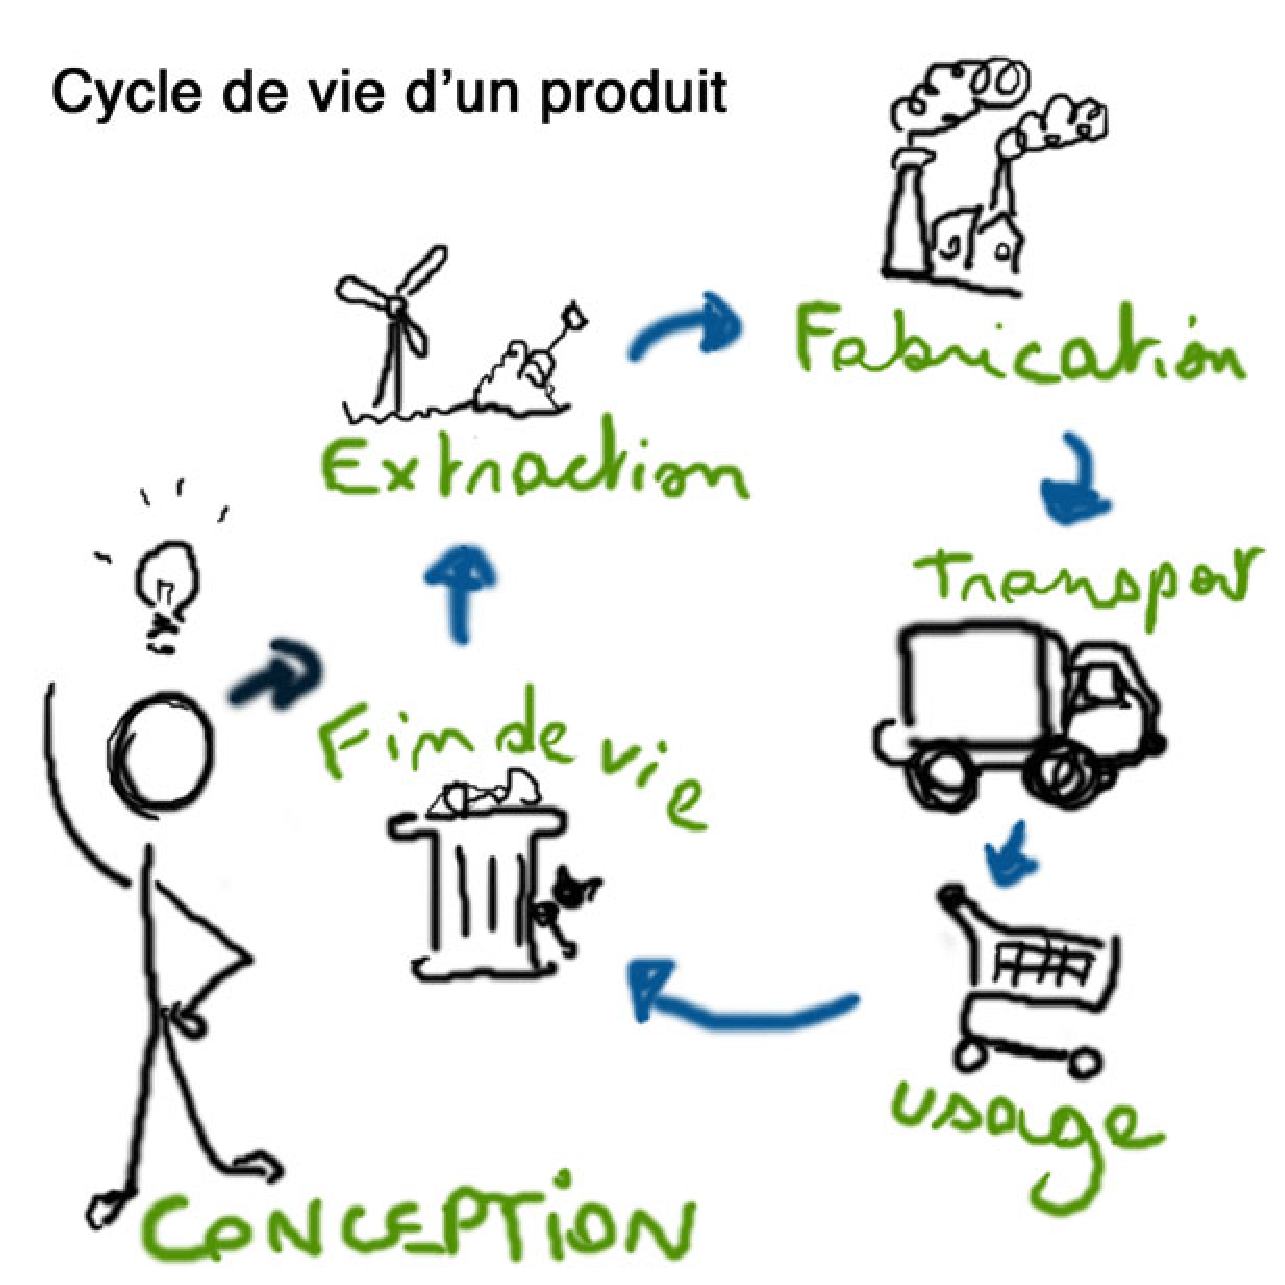
\includegraphics[width=0.6\textwidth]{figures/Cycle-de-vie}
	\caption{Cycle de vie (source ~: wikipedia, auteur ~: DamarisBasileJudith)}
	\label{CdV}
\end{figure}

La particularité du produit qu'est le logiciel par rapport aux produits standards de l'industrie (la dématérialisation en particulier) fait qu'il est difficile d'appliquer un modèle existant pour effectuer une ACV d'un logiciel. Il serait donc nécessaire de travailler à l'élaboration d'un modèle propre au logiciel.
			\subsubsection{}
			
		
	\section{La mesure de consommation d'énergie}
Dans cette partie de l'état de l'art je vais parler des différentes techniques pour extraire et utiliser une information sur la consommation d'un logiciel.
		\subsection{Différentes approches pour mesurer la consommation des ressources}
J'ai pu identifier trois méthodes différentes pour mesurer l'énergie consommée. Elles ont chacunes leurs avantages et leurs défauts.
			\subsubsection{La mesure par un appareil externe}
La première méthode, la plus commune pour mesurer les resources consommées par un appareil électrique, est de placer un wattmètre en série sur l'alimentation de cet appareil. Avec un wattmètre récent on peut mesurer un ensemble de paramètre tels que les watts, les watts/heure, les volts et les ampères. De plus, la plupart des outils récents proposent un système d'enregistrement et/ou de transfert des données vers un ordinateur.

\begin{wrapfigure}{dR}{0.3\textwidth}
		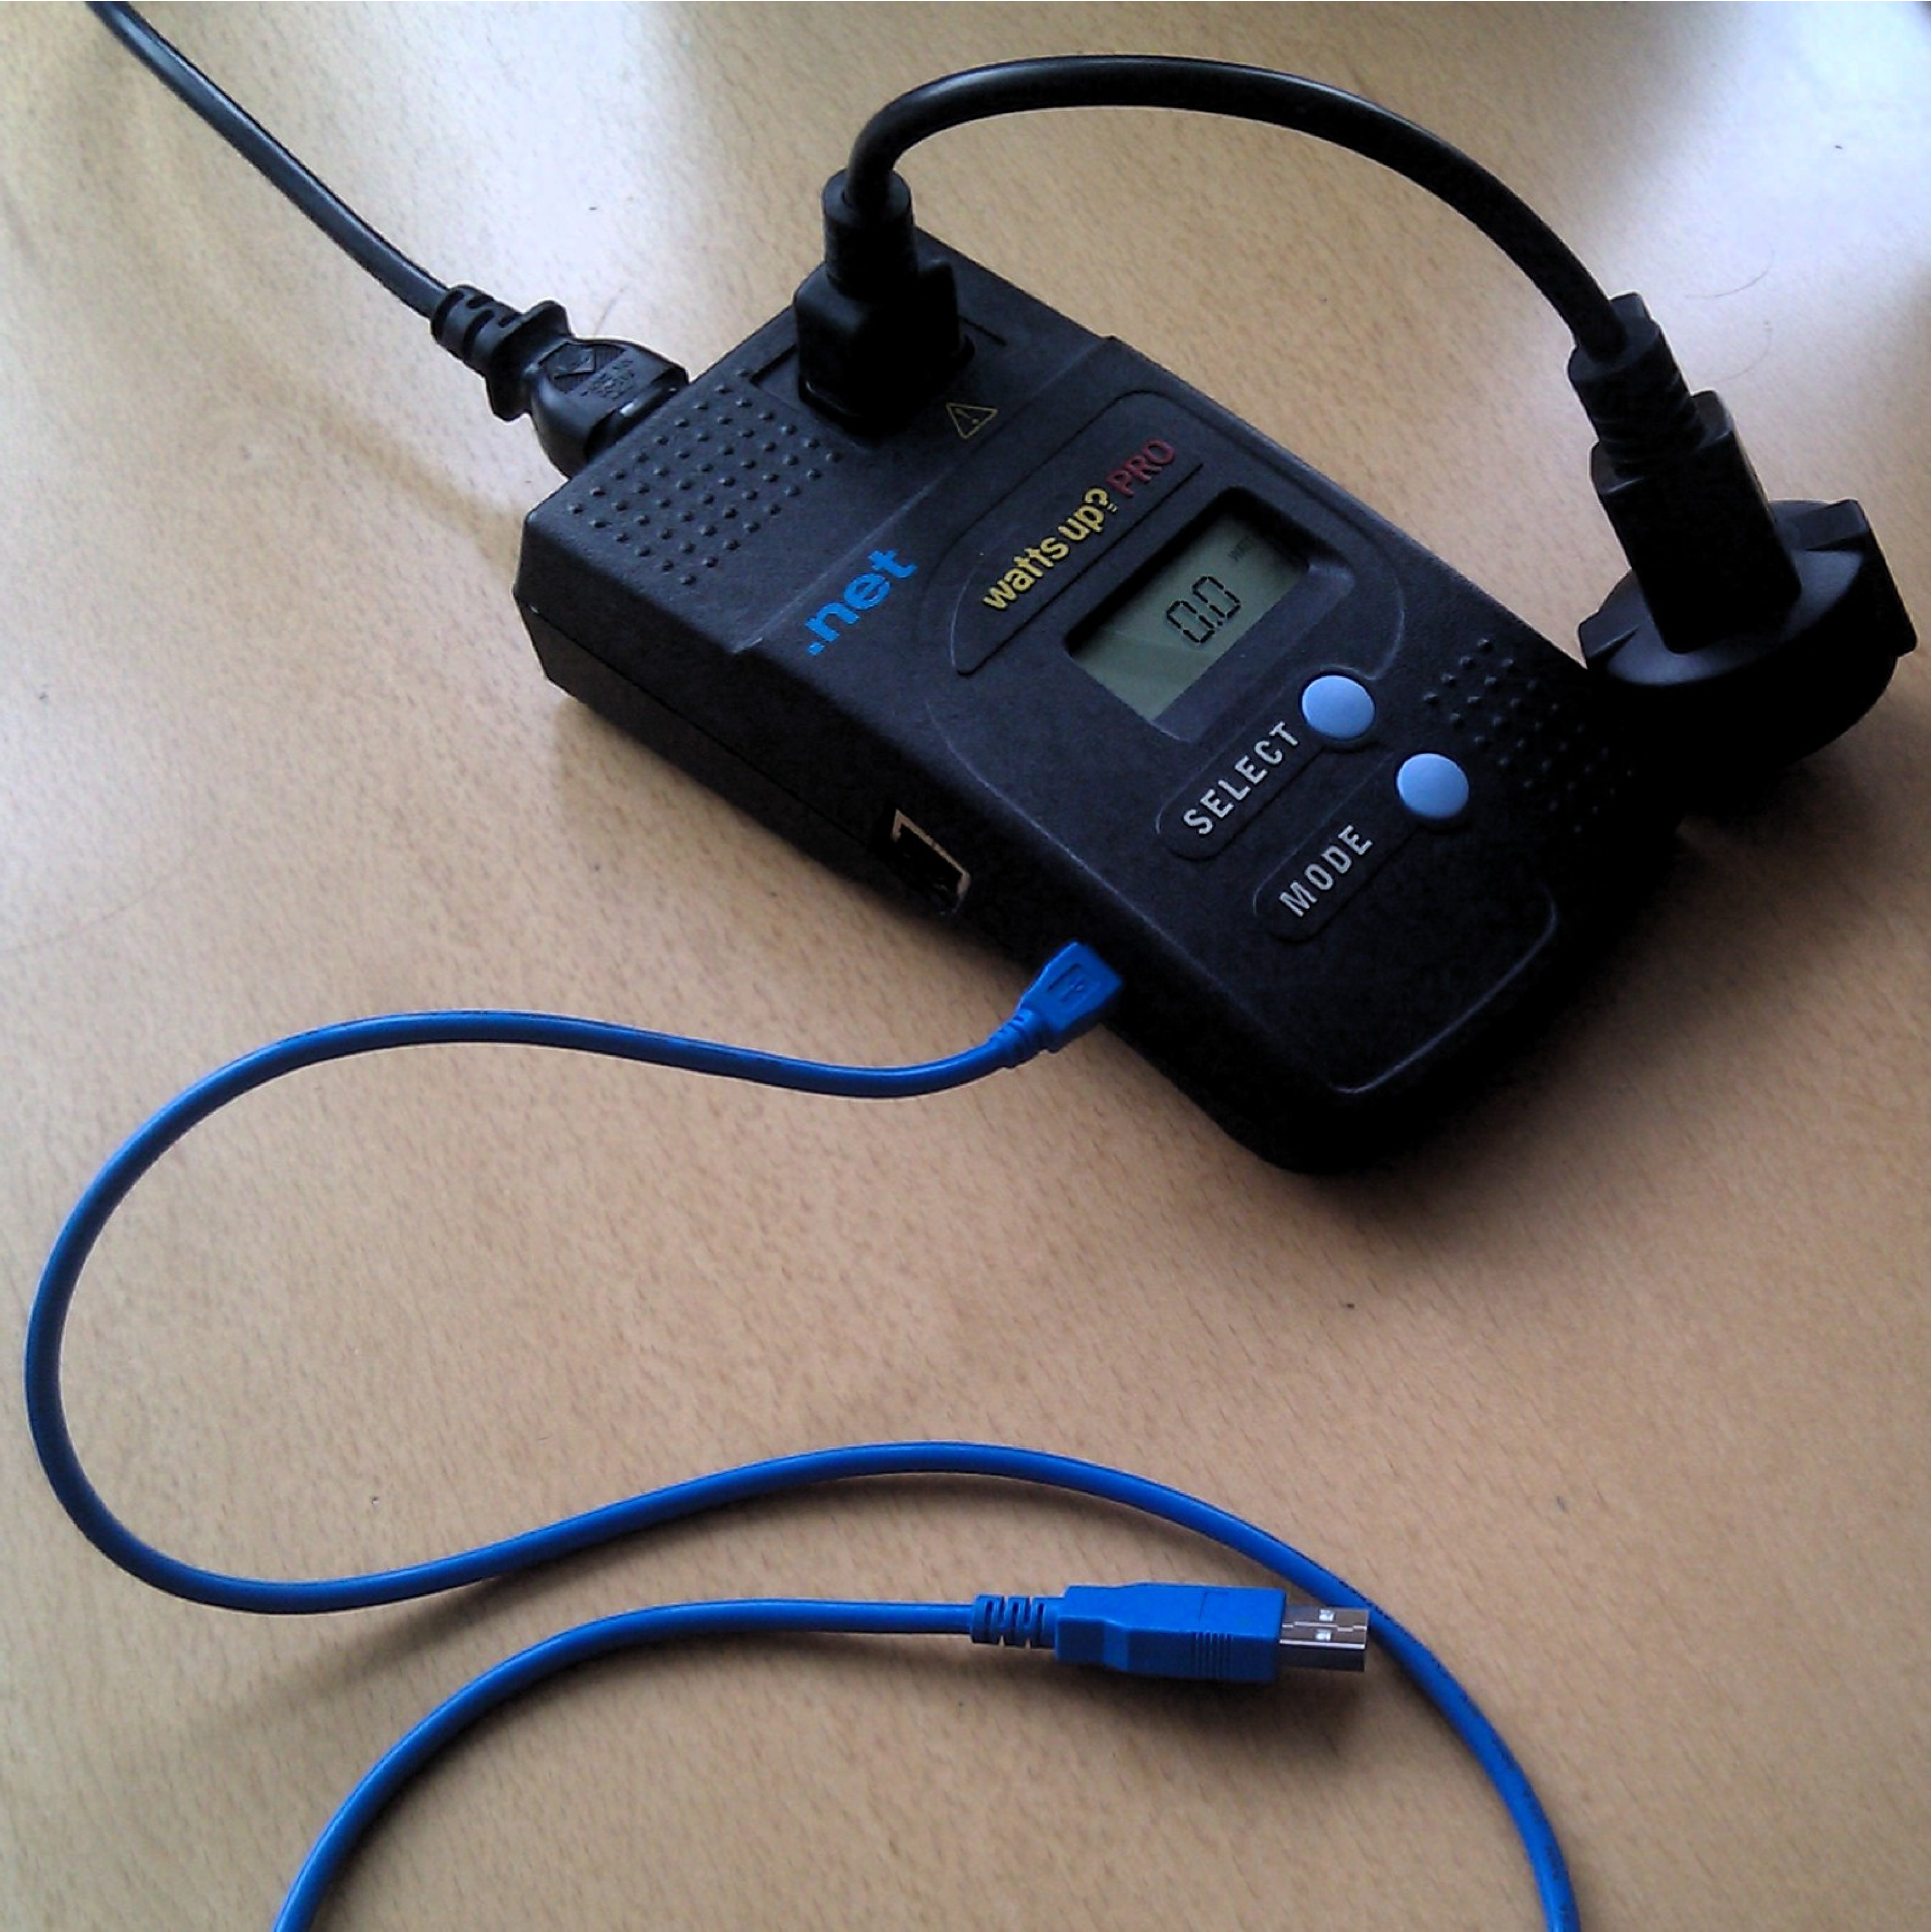
\includegraphics[width=0.3\textwidth]{figures/wattsUp}
		\caption{Photo d'un watts up pro .net}
		\label{wattsUp}
\end{wrapfigure}

Par exemple, les \textit{plugwizes} sont des modules qui se placent sur la prise sont capables de couper l'alimentation de l'appareil branché dessus et de mesurer la consommation électrique de celui ci. Ils sont capable de transmettre ces informations sans fil jusqu'à un ordinateur. Un autre exemple de ce type de matériel, les wattmètres de la marque \textit{watts up\/?}. Ils permettent, suivant leur gamme, de collecter de l'information et de la transmettre. Le \textit{watts up\/? pro .net} (figure~\ref{wattsUp}) dispose d'un système d'enregitrement de, au maximum, 120000 mesures de watts et de deux interface de communication, USB et Ethernet.

Cette technique de mesure n'offre qu'une vue globale de notre système. Il est impossible par cette méthode d'identifier de manière certaine la consommation d'un logiciel. On peut par contre corréler un changement de consommation avec un événement survenu\cite{GreenMining} (le démarrage d'une application, le lancement d'une tâche gourmande en traitement\ldots). 

			\subsubsection{La mesure par un logiciel interne}
La deuxième méthode consiste à analyser les ressources utilisées par un programme et, à partir d'un modèle de consommation, d'en déduire la consommation énergétique de l'application. Différentes ressources peuvent être ciblées. On peut les classer en deux catégories ~: les unités de calcul (CPU, GPU\ldots) et les dispositifs d'entrées/sorties (disque dur, interface réseau\ldots).

Dans cet article\cite{noureddine:hal-00681560}, les auteurs détaillent le modèle de consommation qu'ils ont mis au point pour leur application de mesure PowerAPI. On peut y voir qu'ils obtiennent des résultats intéressants par rapport à la mesure faite en parallèle sur un wattmètre. L'inconvénient de ce type de méthode est qu'il faut calibrer le modèle. Cela est nécessaire car chaque processeur  fonctionne différemment et donc ne consomme pas la même chose. De plus ce type de méthodes est intrusive et peut perturber le fonctionnement du logiciel.

En revanche cette technique permet facilement d'isoler un logiciel en particulier (ou plutôt un processus). C'est donc une technique intéressante pour mon projet.

			\subsubsection{Vers une mesure par un appareil interne}
Enfin une troisième technique est à envisagé dans un futur plus ou moins proche. Comme l'explique l'article \textit{Looking back on the language and hardware revolutions
~: measured power, performance, and scaling}\cite{Esmaeilzadeh:2011:LBL:1950365.1950402}, les fabricants de matériel intègrent, de plus en plus, dans leurs composants, des mécanismes de mesure afin d'adapter leurs fonctionnements à leurs consommations. À la fin de l'article, les auteur recommande l'ouverture de ces mécanismes au travers d'API pour que les développeur puissent y accéder.

Si les constructeurs acceptent de faire cet effort, on pourra facilement savoir ce que consomme réellement une application en temps réel. Ce type de mécanisme serait idéal dans mon projet car il permettrait d'avoir une consommation réelle de l'application mesurée. On pourrait même concevoir, très facilement, des applications qui s'adaptent en fonction de leur consommation.

%		\subsection{Comment comparer la consommation de deux logiciels}
%TODO écrire la subsection Comment comparer la consommation de deux logiciels
%TODO chager le titre Comment comparer la consommation de deux logiciels
%			\subsubsection{Deux versions d'un logiciel}
%Article Green mining\cite{GreenMining} décrivant une méthodologie

%			\subsubsection{Deux logiciels isofonctionnel}
%Parler des métriques.

%			\subsubsection{Deux logiciels diférents}
%Parler de métrique plus complexe.
		
	\section{Fabriquer un éco-logiciel}
Cette partie ne va pas expliquer comment fabriquer à coup sûr un éco-logiciel. Je souhaite seulement y présenter certains concepts importants pour appliquer le développement durable au logiciel.
		\subsection{De la Conception\ldots}
La conception d'un éco-logiciel doit être particulièrement bien pensée. C'est lors la conception que l'on prend la majorité des décisions qui entraineront une sur-consomation par la suite. Il m'est difficile de lister l'ensemble des questions à se poser lors de cette phase. Je ne citerais que quelques points importants.

La première question à se poser est celle de l'architecture et de la localisation des traitements\cite{EcoLogiciels}. Des traitements effectués dans un Centre de données auront un coup plus faible car un centre de données dispose souvent de mécanisme d'optimisation énergétique. Une autre question importante à se poser, est celle de la configuration par défaut\cite{GreenPattern}. En effet, une majorité d'utilisateurs laisseront l'application avec son mode de fonctionnement par défault.

On pourait dresser une liste importante de ce qu'il faut ou ce qu'il ne faut pas faire. En résumé, il faut réfléchir en terme d'écologie chaque choix  fait durant la conception.

		\subsection{\ldots~À la programmation}
La programmation d'application \og verte \fg est encore plus dur à définir que la conception. Il n'y a pas de méthode miracle. Il faut avoir une bonne connaissance du langage, bien choisir les mécanismes utilisés (boucle, saut conditionnel\ldots). Le plus simple ici est de s'assister d'outils d'aide à la programmation. Il n'en existe pas encore de suffisament évolué dans l'éco-conception, mais beaucoup d'optimisation proposée par des outils comme Sonar\footnote{http://www.sonarsource.org/} réduisent l'empreinte énergétique d'un code.

Ensuite, je dirais que l'expérimentation peut permettre de trouver des amélioration dans un code (dépliage de boucle, organisation des données\ldots).
		\subsection{La programmation Modulaire}
			\subsubsection{Intéret de la programmation modulaire dans l'économie d'énergie}
La programmation modulaire présente beaucoup d'avantage pour l'éco-conception de logiciel. Dans l'absolu, un programme modulaire est plus facile à maintenir et a une durée vie potentiellement plus longue qu'un programme standard. Comme ses modules sont indépendant les uns des autres, il suffit de remplacer la brique deffectueuse pour réparer un problème. De même, l'évolution du programme se fait par l'ajout de nouvelles briques.

D'autres aspects intéressants pour l'éco-conception sont à prendre en compte. Si dans une application modulaire l'utilisateur ne se sert pas de toutes les fonctionnalités, on doit pouvoir retirer les modules qui ne servent à rien. Cela peut potentiellement économiser de l'énergie à l'exécution mais surtout alléger considérablement le logiciel et donc allonge la durée de vie de l'ordinateur.

			\subsubsection{OSGi ~: du java modulaire}
OSGi\footnote{Open Services Gateway initiative} est une cadriciel java élaboré par l'OSGi Alliance. C'est un consortum formé en 1999 composé entre autre d'IBM, Motorola,Oracle ou encore Samsung. Le but de ce cadriciel est de faciliter la création d'application modulaire en Java. 

Différentes implémentations de ce framework ont été développés à partir de la spécification produite par l'OSGi Alliance. Les plus connu sont Equinox développé par l’équipe du projet Eclipse, Felix issu du projet universitaire Oscar et maintenu par Apache ou encore Knopflerfish élaboré par MakeWave.
		
	\section{Travaux connexes}
Dans cette section je vais présenter les projets en rapport avec mon sujet de stage et dont j'ai soit entendu parlé soit pu rencontrer les acteurs.
		\subsection{Le Green code Lab}
Le green code lab est un groupement de personne souhaitant promouvoir le développement durable dans le logiciel. C'est une communauté virtuelle qui se charge de publier des articles d'informations, d'organiser des évenements et des formation autour de l'éco-conception de logiciel.

Leur site internet (\href{http://www.greencodelab.fr}{www.greencodelab.fr}) sert de plateforme de publication de leurs articles. Ils ont aussi mis en place un GitHub qui sert de laboratoire pour effectuer des expérimentations. Enfin le green code lab a publié un livre intitulé \textit{Green Pattern - Manuel d'éco-conception des logiciels} et disponible à la vente au format papier ou numérique.

Durant mon stage, j'ai eu l'occasion de me rendre à l'un de leurs évenements sur le thème de la mesure de la consommation électrique d'un logiciel. Là-bas, Olivier Philippot, un membre actif du green code lab, nous a présenté une méthodologie basée sur des \textit{plugwizes} en affichant les mesures au moyen du logiciel KST\footnote{http://kst-plot.kde.org/}{kst-plot.kde.org/}.
		\subsection{Le projet code vert}
Code Vert est un projet labélisé par le pôle de compétitivité Images et Réseaux qui a débuté en Février 2012 (en même temps que mon stage) est durera 2 ans. Il regroupe 4 acteurs ~: l'école d'ingénieur ICAM, les sociétés KaliTerre et TOCEA, ainsi que la ssii SIGMA Informatique.

L'objectif de ce projet est de mettre en place un référentiel pour juger de l'éco-conception du code d'un logiciel. Cela passera par une analyse statique du code qui sera noté. On pourra ressortir de cette analyse des recommandations qui permettront de l'améliorer.
		
	\section{Conclusion}
Voici que se termine mon état de l'art. Avec les connaissance présenté dans ce chapitre j'ai pu réaliser un certain nombre de choses que je vais maintenant présenter.

\chapter{Comment peut-on mesurer la consommation d'un logiciel ?}
Dans ce chapitre je ne vais m'intéresser qu'à la consommation du logiciel lors de l'exécution. Je ne prendrai pas en compte les différentes étapes du cycle de vie.
	%\section{Qu'est ce qui consomme dans un ordinateur ?}
	%TODO écrire la section Qu'est ce qui consomme dans un ordinateur ?
	\section{Outils de mesure de la consommation des ressources par un logiciel}
Voici l'ensemble des logiciels que j'ai pu expérimenter pour mesurer la consommation énergétique d'un programme. Pour chacun je note mes observations sur son fonctionnement, son installation ou toute autre remarque pouvant servir.
		\subsection{Ptop}
pTop est un programme de collecte d’information sur l'exécution de processus sous linux. Il est censé récupérer les données sur l'utilisation du CPU, de la RAM et des échange réseaux. Il doit ensuite être capable, une fois le modèle paramétré, sortir des informations sur la consommation énergétique.

Malheureusement, il s'est avéré que pTop ne fonctionne pas entièrement. Après plusieurs essais infructueux, j'ai supposé que le logiciel avait été abandonné sans être fini.

			\subsubsection{Procédure d'installation}
\begin{itemize}
    \item récupérer les sources sur http://mist.cs.wayne.edu/ptop.html
    \item installation du nécessaire pour compiler les sources (paquets debian) ~:
    \begin{itemize}
	\item build-essential
	\item libmysqlclient-dev
	\item libncurses-dev
    \end{itemize}
    \item Installation de la base de données Mysql ~:
    \begin{itemize}
	\item création d’une base de donées ptop
	\item exécution du script db\_schema.sql
	\item remplacement du login et password pour accéder à la base de données dans le fichier database.c
    \end{itemize}
    \item Compilation ~:
\end{itemize}

\begin{verbatim}
	# make
	# chmod +x ptop
\end{verbatim}

\subsubsection{Exécution}
Lancer le programme au moyen de la commande ~:

\begin{verbatim}
# ./ptop
\end{verbatim}

Le programme va s'initialiser et enregistrer les mesures dans les bases de données. Il faut ensuite interrompre les mesures au moyen du signal SIGINT.

\subsubsection{Données de sortie}
Il n’existe pas, à ma connaissance, de documentation précise sur les données de sortie du programme pTop.  Le programme stocke les données dans une base de données Mysql nommé ptop. Elle est composée de quatre tables ~:
\begin{itemize}
	\item device\_energy
	\item process\_energy
	\item process\_info
	\item sys\_info
\end{itemize}

Seules les deux dernières tables sont remplies par le programme (à cause soit d’un bug, soit d’une version non fini du programme).

\subsection{Energy Checker}
Le projet Energy Checker développé par Intel, est un ensemble d’outils destiné à faciliter la remontée et l’affichage des mesures faites sur la consommation d’un programme. Il se compose principalement de l’API Energy checker qui permet d’utiliser les mécanismes de remonter d’information (PL - Productivity Link)

\subsection{ClassMexer}
ClassMexer est un API java permettant d’estimer la taille en mémoire d’un objet java. On peut télécharger cet API sous la forme d’un fichier JAR à cette adresse ~: http://www.javamex.com/classmexer/. ClassMexer est un Instrumentation agent comme spécifié dans le pattern Instrument. Cela implique de travailler avec, au minimum, la version 5 de java.

\subsubsection{procédure d'installation}
\begin{itemize}
	\item Télécharger l’API
	\item Importer le fichier JAR dans le projet.
	\item Insérer des appels sur l’objet que l’on souhaite mesurer. Par exemple ~:
\begin{verbatim}
public class Main {
	public static void main(String[] args) {
		String str = "Hello world !";
		
		long noBytes = MemoryUtil.deepMemoryUsageOf(str);
		
		System.out.println(noBytes);
	}
}
\end{verbatim}
	\item Exécuter le programme avec l’option -javaagent:<fichier JAR>
\end{itemize}

\subsection{JouleMeter}
Joulemeter est un outil développé par Microsoft et qui sert à mesurer la consommation d’énergie sur un ordinateur. Il ne fonctionne que sous Windows 7.

\subsubsection{Procédure d'installation}
\begin{itemize}
	\item Télécharger le logiciel sur ce site ~: Joulemeter
	\item Exécuter le programme.
\end{itemize}

\subsubsection{Fonctionnement}
Joulemeter est un logiciel de mesure qui se base sur un modèle de consommation. La première étape est donc de générer ce modèle. Deux méthodes existent.

La première n’est utilisable que sur un ordinateur portable muni d’une batterie. Il suffit de débrancher l’alimentation et de lancer la calibration (15 minuntes sans utiliser le PC). Avant de lancer la calibration, il faut faire attention à arrêter toutes les applications afin que le logiciel puisse déterminer une consommation minimum en mode "Idle".

Le deuxième mode nécessite un Wattmètre WattsUp pour générer le modèle. Il suffit de le brancher en USB, de couper toutes les applications possibles et de lancer la calibration (3 minutes sans utiliser le PC).

\subsubsection{Expérience}
Afin de tester la fiabilité du modele créé, j'ai effectué différentes expériences en comparant les résultats obtenu par Joulemeter avec ceux lu sur un wattmètre. J'ai pu mettre en évidence de grosses faiblesses qui rendent peu fiable les résultats obtenu. La figure~\ref{joulemeter} met en évidence ces faiblesses. J'ai obtenu ces mesures en laissant fonctionner Joulemeter sur un ordinateur, démaré mais inutilisé, durant toute une nuit. En parallèle, j'ai récupéré les mesures que prenait un wattmètre \textit{WattsUp pro}.

\begin{figure}
	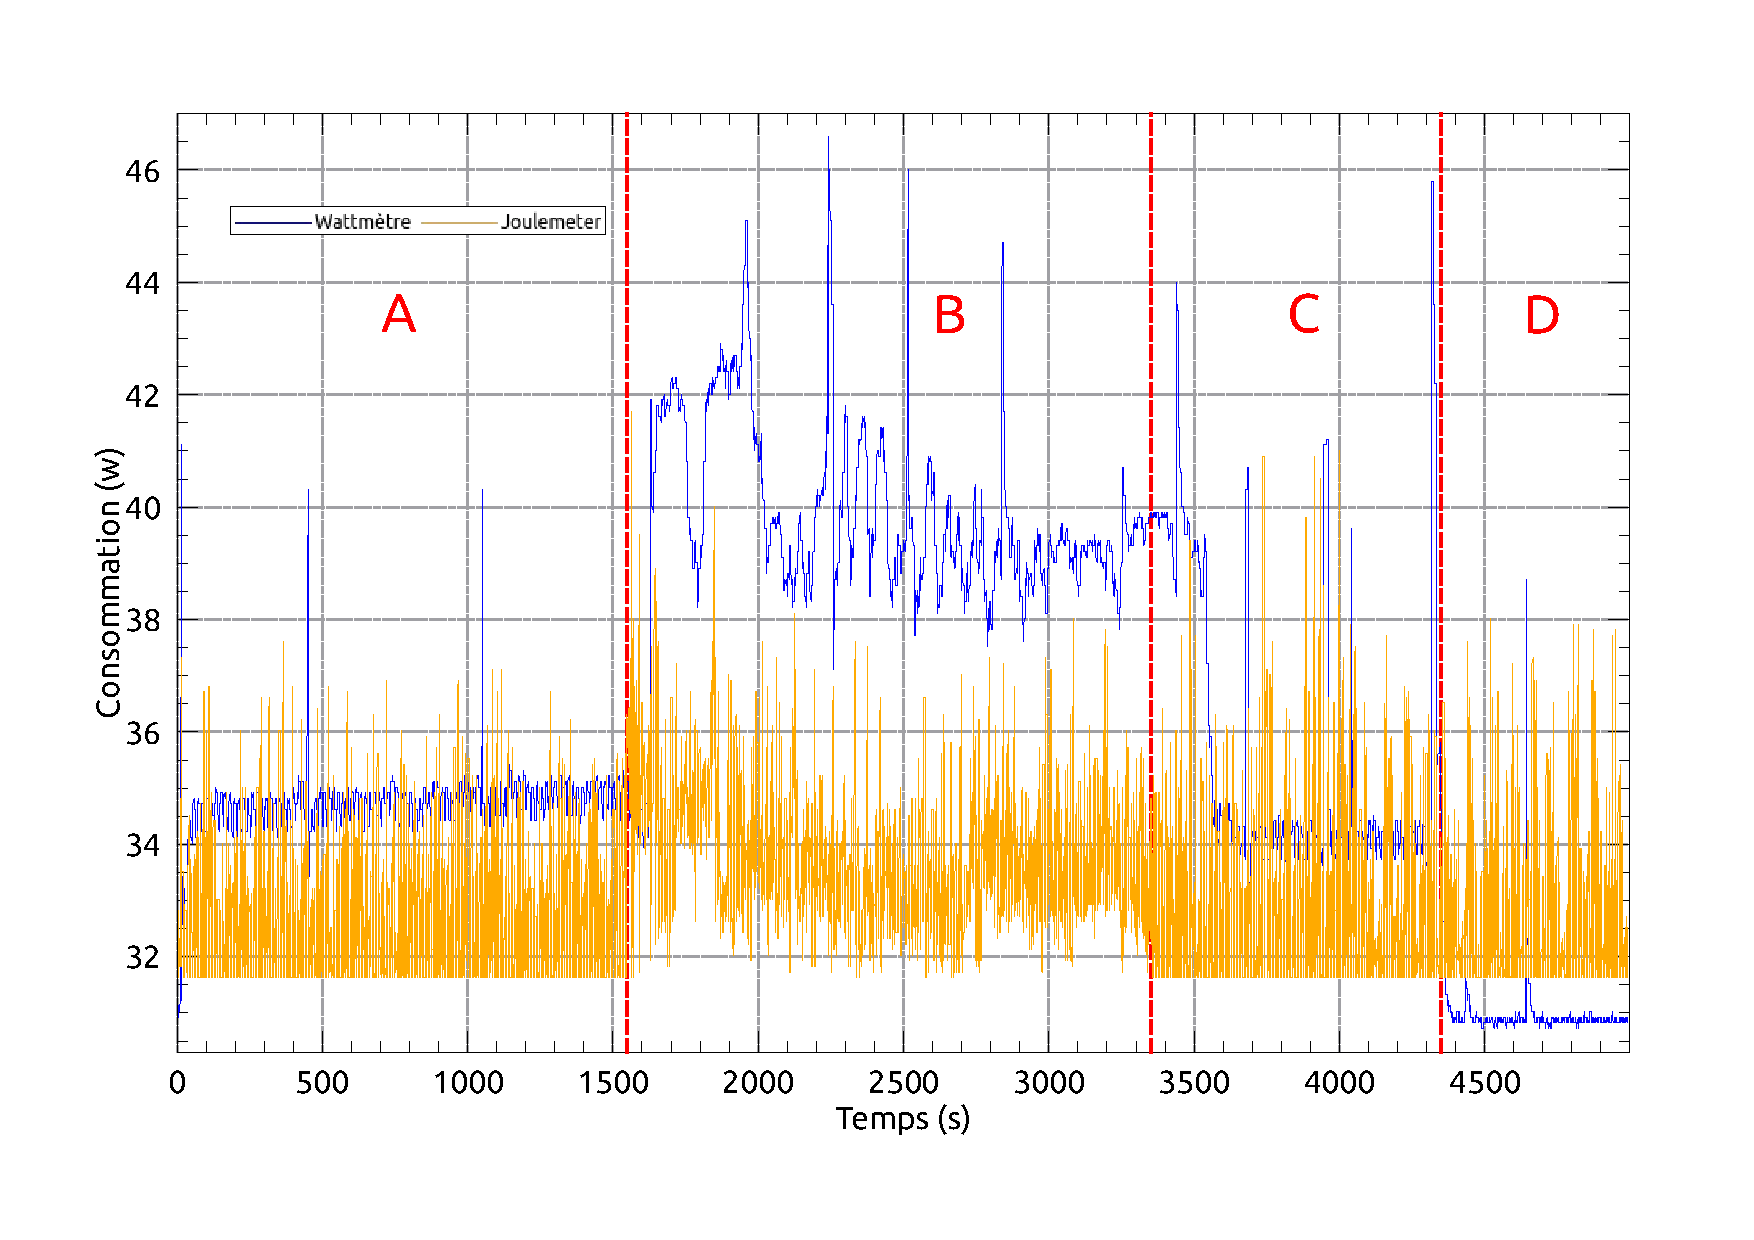
\includegraphics[width=0.99\textwidth]{figures/joulemeter.pdf}
	\caption{Mesures faites par Joulemeter comparé à celles d'un wattmètre}
	\label{joulemeter}
\end{figure}

Les deux coubes affichent un échantillon  de 5000 mesures (durant approximativement 5000 secondes). Le modèle de consommation sur lequel se basait Joulemeter a été généré juste avant le début de l'expérience. D'un point de vue général, on peut déjà remarquer que la courbe de Joulemeter est très irrégulière et majoritairement en dessous de celle du watttmètre. Cela est principalement du, au fait que l'impact du processeur est largement sous-estimé dans le modèle.

Ensuite on peut noter un seuil en dessous du quel joulemeter ne descend pas (ici, 31,6 watts). On constate même que les mesures du wattmètre passe en dessous de celle de joulemeter dans la partie \textit{D} du graphique. Cet effet de seuil est engendré par le modèle qui considère que le système consomme toujours une constante quand il est allumé. Donc, quelle que soit la charge du système, Joulemeter considère qu'il consomme au minimum 31,6 watts (valeur qu'il a mesuré lors de l'établissement du modèle).

Enfin, et tout n'est pas négatif, on peut remarquer que dans la zone B Joulemeter réussi à mesurer une hausse de la consommation qui peut être noté sur la courbe du wattmètre (avec un certain décalage cependant).

\subsection{PowerAPI}
PowerAPI est un outil sur lequel travail l'équipe ADAM de l'université de Lille. Les premiers résultats de cet outil ont été présentés dans un papier\cite{noureddine:hal-00681560} publié à l'ICSE\footnote{International Conference on Software Engineering} 2012 à Zurich. Cet outil parait prometteur et s'il continue à être développé, pourrait bien apporter une solution intéressante au problème de la mesure de consommation énergétique de logiciel.

Selon la présentation qui en a été faite, il fonctionne actuellement pour la consommation CPU. Cet outil collecte le temps CPU d'un processus et la fréquence de celui-ci en temps réel. Puis il détermine l'énergie consommée grâce à des tables de consommations par rapport à la fréquence fournis par les fabriquant de processeur.

Je n'ai malheureusement pas essayé PowerAPI par manque de temps. Je n'ai eu accès au programme que tardivement durant mon stage et à ce moment je travaillais sur d'autres aspects.

%\chapter{Mise en valeur de l'impact du code sur la consommation}
%TODO écrire le chapitre Mise en valeur de l'impact du code sur la consommation
%Tout au long de mon stage j'ai développé un ensemble de petits programmes qui mettent en valeur une bonne pratique à adopter, la faiblesse d'un mécanisme ou encore l'importances des choix effectué durant le développement d'un logiciel. Dans ce chapitre je vais présenter les exemples les plus éloquants. 
%	\section{Impact du choix du langage}
%	\section{Impact des choix de programmation}
%		\subsection{Description des tests}
%		\subsection{Resultats obtenus}

\chapter{La programmation modulaire au service de l'économie d'énergie}
Afin de mettre en valeur l'importance de l'architecture logicielle dans la consommation, j'ai proposé de développer une application basée sur la technologie java OSGi\footnote{\href{http://www.osgi.org}{www.osgi.org}}. L'objectif de ce projet est de pouvoir réaliser facilement des démonstrations d'application modulaire qui s'adapte en fonction de contrainte énergétique. J'ai donc choisi d'élaborer un cadriciel qui permettrait d'échanger une partie de l'application (dans notre context un \og bundle \fg OSGi) contre une autre afin d'optimiser la consommation. Afin d'expliquer plus clairement le but du projet, je vais détailler un cas d'utilisation du cadriciel.

Un programme doit réaliser une tache. Le développeur connait deux algorithmes pour coder cette tache. Ils ont chacun leurs forces et leurs faiblesses. La version A du code consomme peu d'énergie en temps normal (figure~\ref{AbsBdlA}). Mais, dans certaines conditions, ici quand un évènement A se produit, l'algorithme se met à surconsommer. La version B du code, elle, consomme plus d'énergie (figure~\ref{AbsBdlB}) que la version A. Par contre il est moins sensible à l'arrivé de l'évenement A. Donc pour réaliser cette tâche en économisant le plus d'énergie il faudrait exécuter le code A en temps normal, et le code B quand l'évenement A se produit. La solution de mettre les deux algorithmes dans le même programme n'est pas une bonne solution. En faisant de la sorte, on alourdit le programme, ce le qui rend plus exigent en ressource et donc avance l'obsolescence des machines. De plus, cela rend la maintenance du code plus difficile.


\begin{figure}
        \begin{subfigure}[b]{0.45\textwidth}
                \centering
                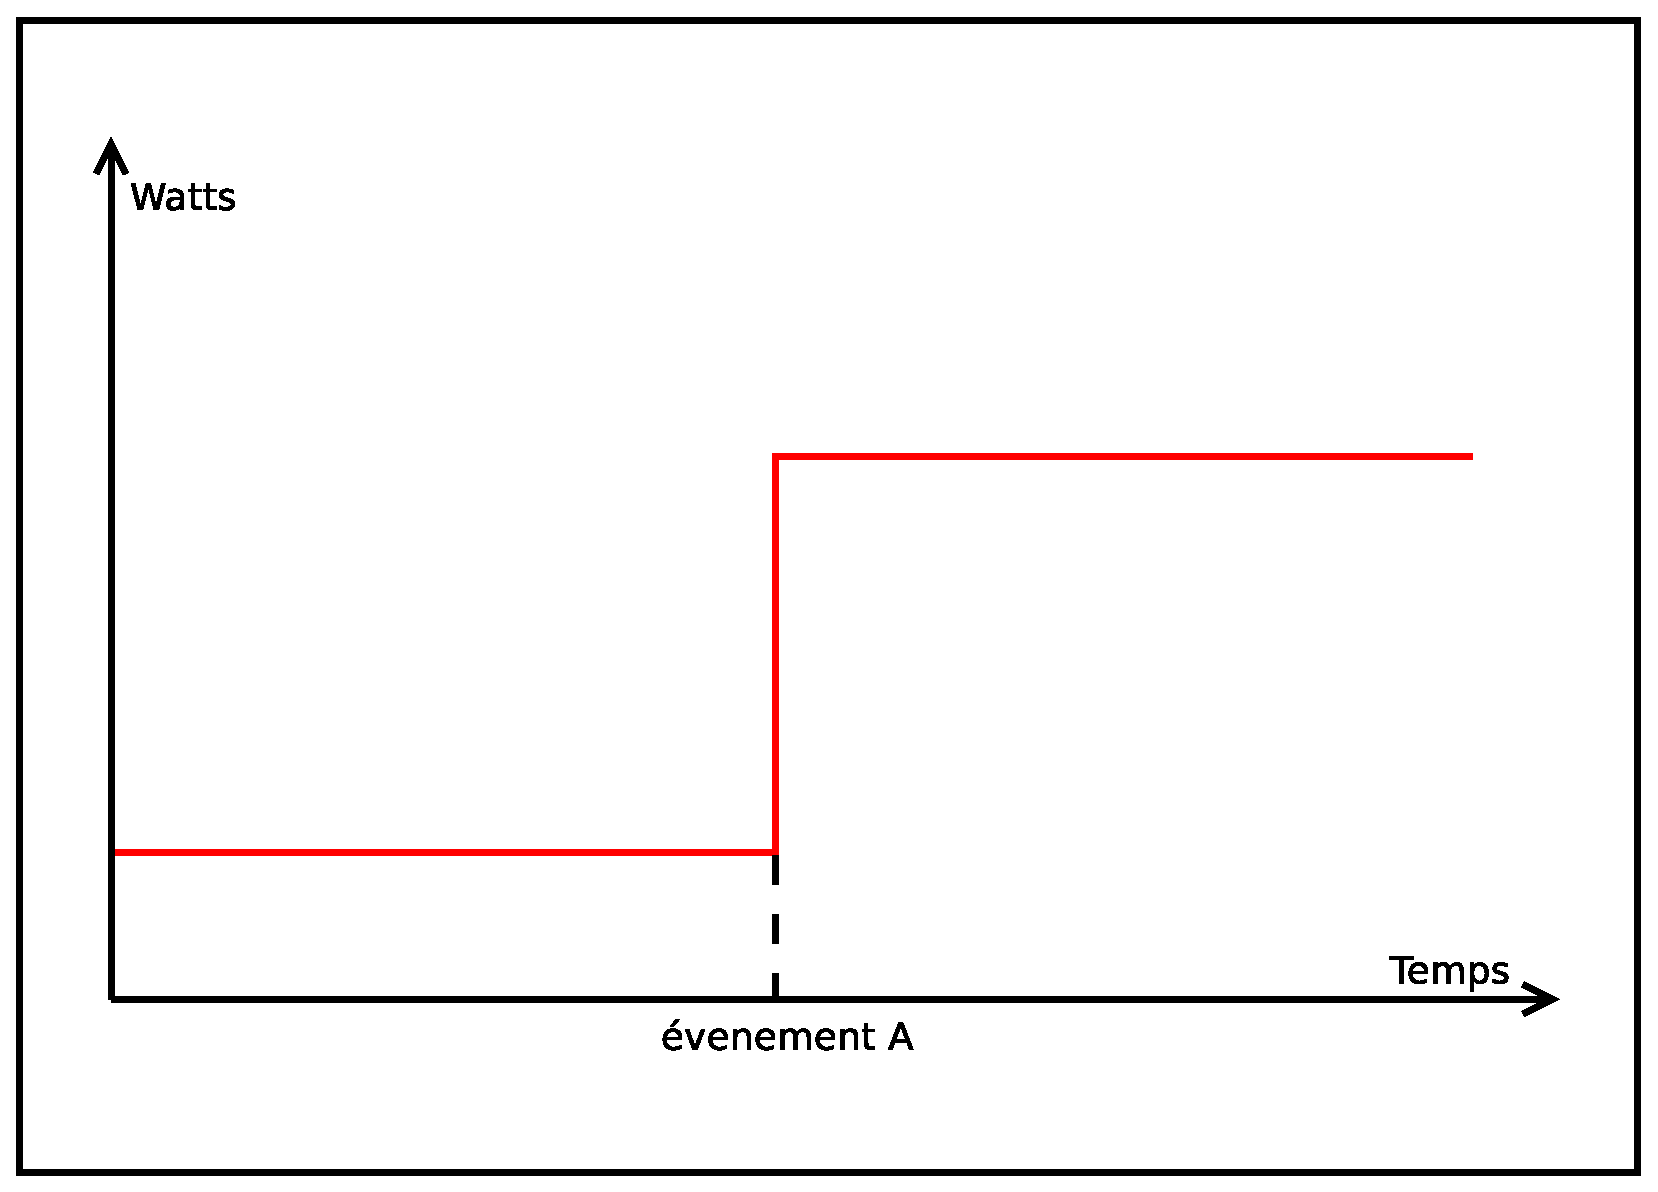
\includegraphics[width=\textwidth]{figures/Abstract_bundle_A}
                \caption{Consommation du module A}
                \label{AbsBdlA}
        \end{subfigure}
        ~
        \begin{subfigure}[b]{0.45\textwidth}
                \centering
                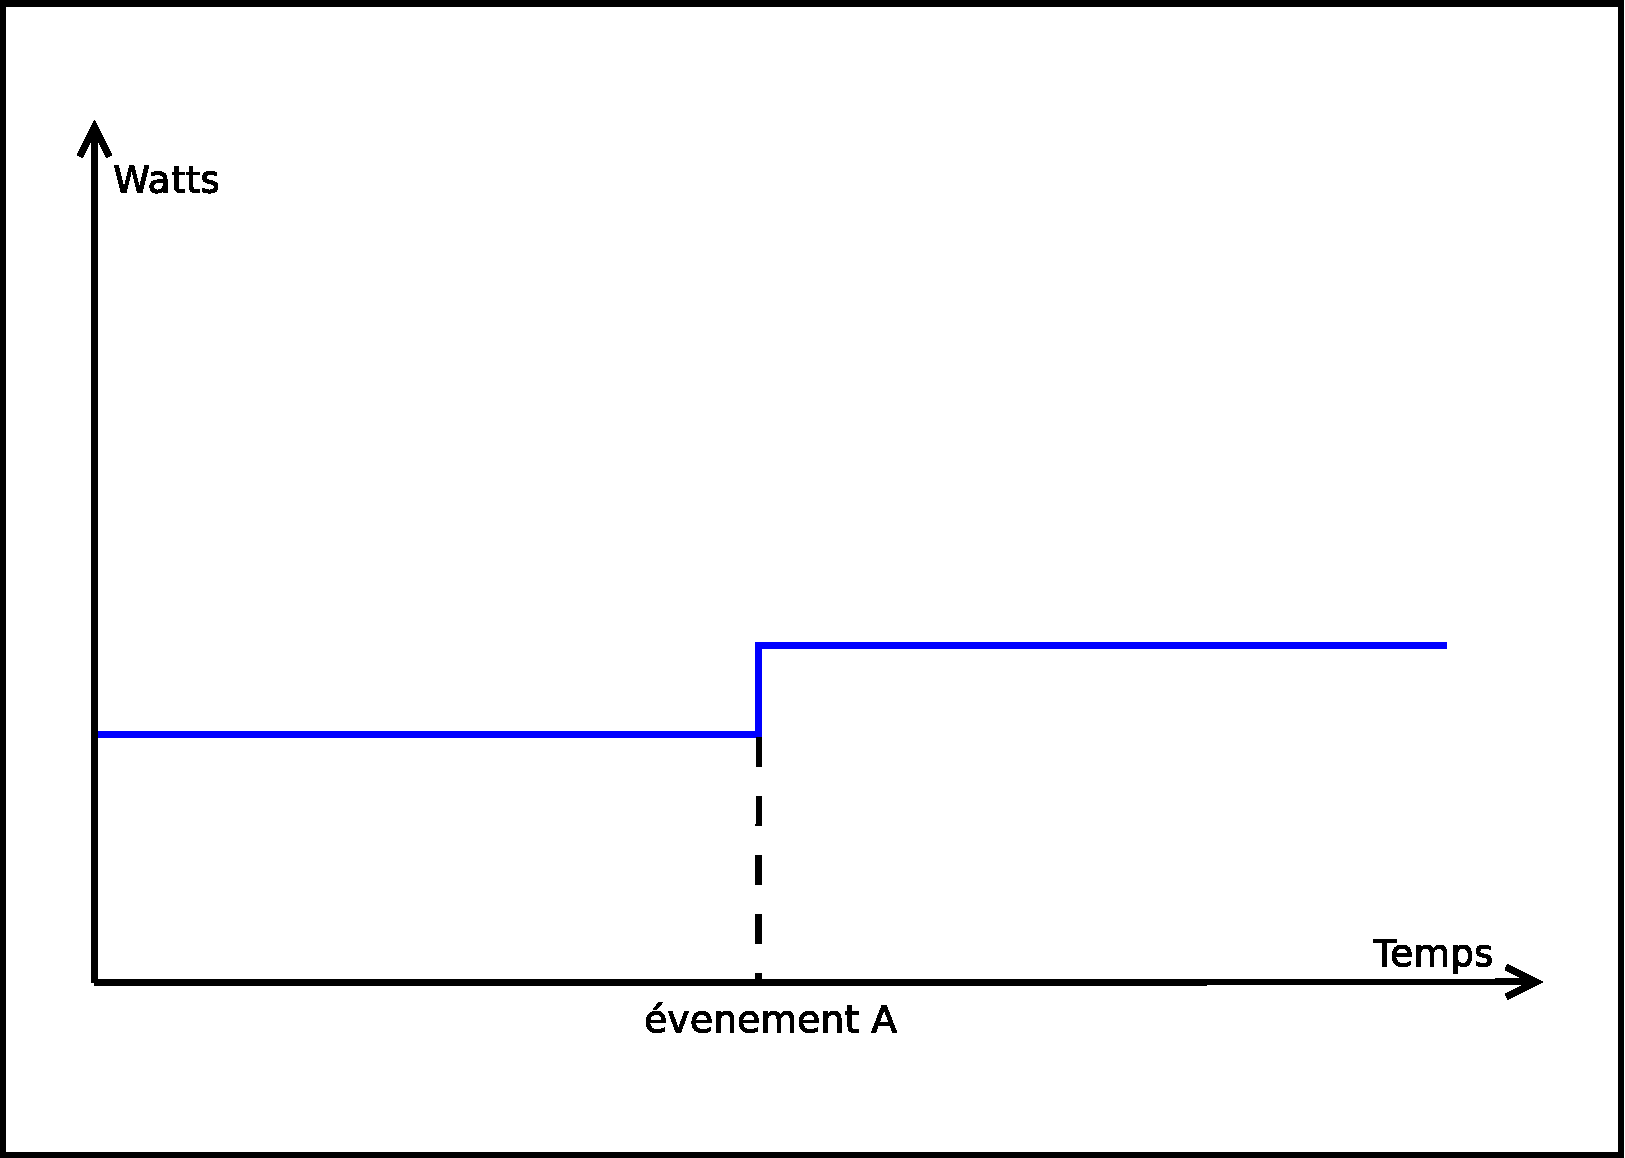
\includegraphics[width=\textwidth]{figures/Abstract_bundle_B}
                \caption{Consommation du module B}
                \label{AbsBdlB}
        \end{subfigure}
        \caption{Illustration de l’optimisation de la consommation par l’échange de module}
        \label{AbsBdl}
\end{figure}

Le cadriciel que j'ai développé a pour but de remplacer à chaud le code A contenu dans un \textit{bundle OSGi} par le code B contenu dans un autre \textit{bundle} lorsque l'évènement se produit. Il y a d'autres cas d'utilisation que l'on pourrait imaginer telle que la mise en place d'une politique énergétique sur une machine (par exemple réduire la consommation d'une machine utilisant l'énergie solaire pendant la nuit).

	\section{Présentation de l'infrastructure développée}
Cette infrastructure est entièrement basée sur OSGi. Elle a donc été conçue sous la forme de modules indépendants les uns des autres. On peut voir sur la figure~\ref{BdlDiag} les modules ainsi que les liaisons entre ces modules. Une flèche d'un module A vers un module B signifie que le module A à besoin de B pour pouvoir fonctionner. Dans cette section je vais détailler l'utilité, voir le fonctionnement de chacun des modules.
	
\begin{figure}
	\centering
	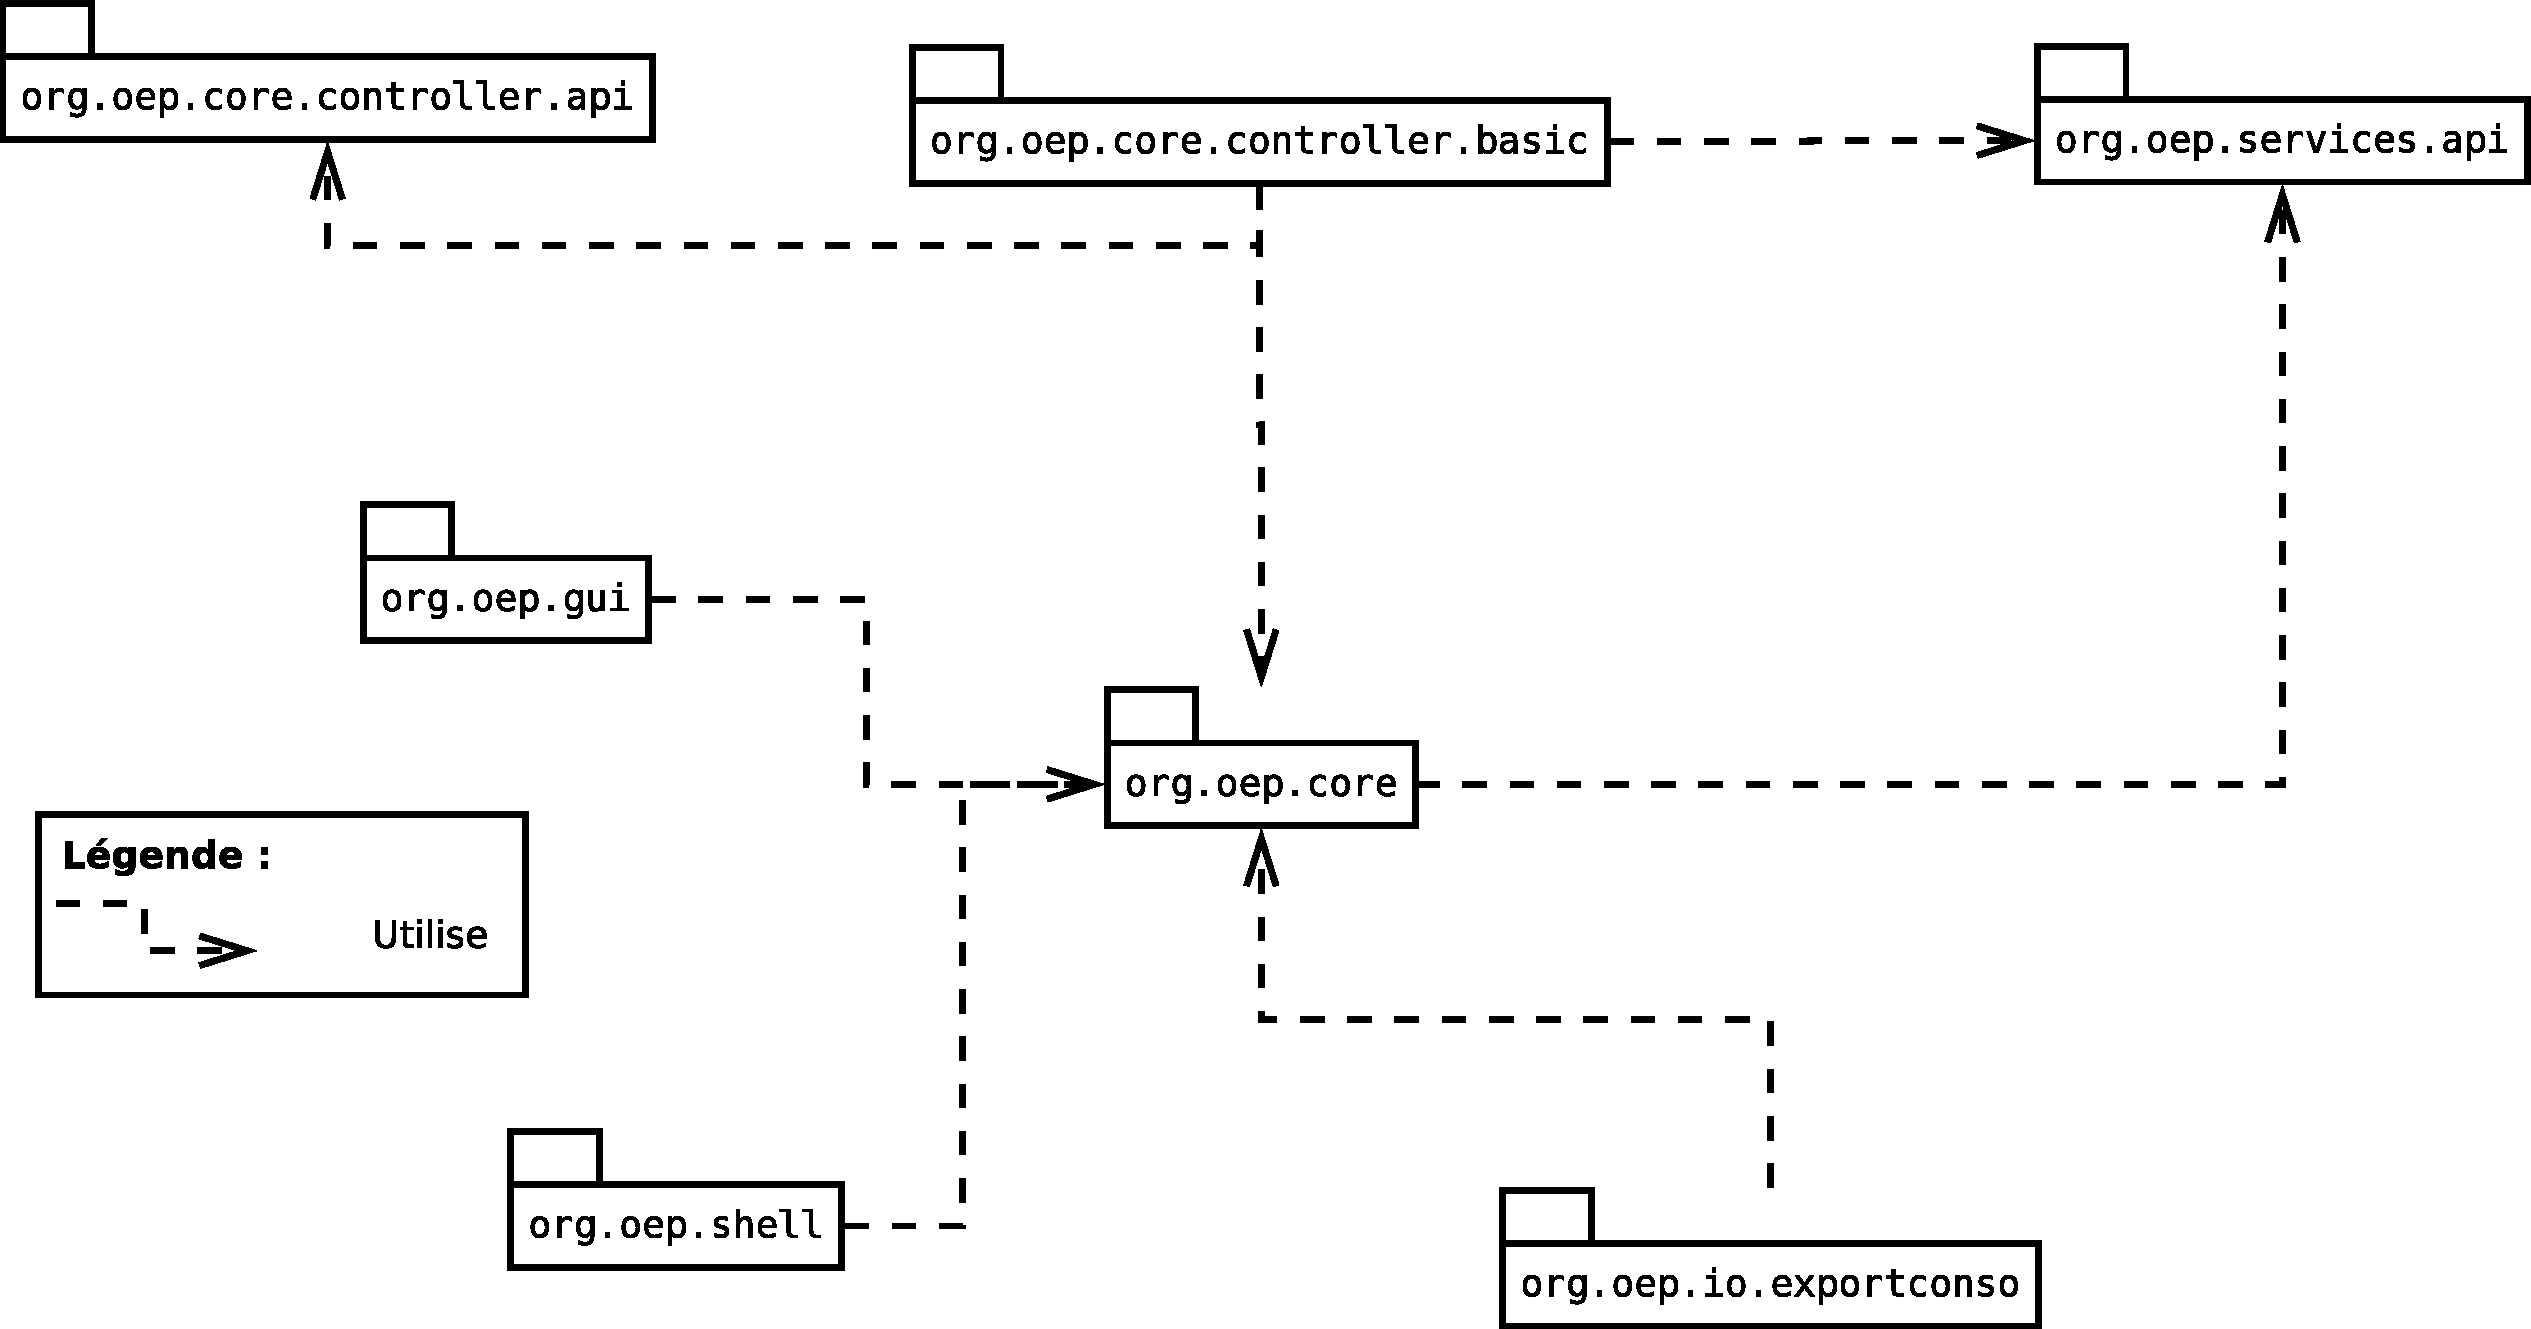
\includegraphics[width=0.95\textwidth]{figures/EcoPattern_Bundle_Diagramme}
	\caption{OSGiEcoFramework ~: diagramme de liaison des modules}
	\label{BdlDiag}
\end{figure}
\subsection{Le coeur du système}
La partie centrale du cadriciel se trouve dans le package \textit{org.oep.core}. Il se découpe en deux classes qui gèrent l'application que l'on souhaite faire fonctionner. La première est la classe \textit{BundleManager}. C'est elle qui s'occupe de gérer les modules qui forment l'application. Elle permet d'installer deux types de modules. Ceux définissant un service et ceux rendant un service. C'est ensuite par cette classe que l'on démarre ou arrête un module offrant un service. Le \textit{BundleManager} garantit qu'il n'y ait qu'un et un seul module démarré par service.

La deuxième classe, \textit{ServiceManager}, s'occupe de référencer les services démarrés. Pour cela elle implémente l'interface \textit{ServiceListener}. Elle permet ensuite de consulter leur consomation au travers de l'interface \textit{EcoService}.
		
		\subsection{Les interfaces}
J'ai développé deux types d'interfaces pour ce framework. Une première graphique, basé sur la technologie \textit{Swing}, l'autre en ligne de commande. L'interface graphique est découpée en deux vues. Une pour installer des services (figure~\ref{BdlList}) et l'autre pour démarrer ou arrêter les services ainsi qu'afficher la consommation (figure~\ref{RngList}).

\begin{figure}
	\centering
	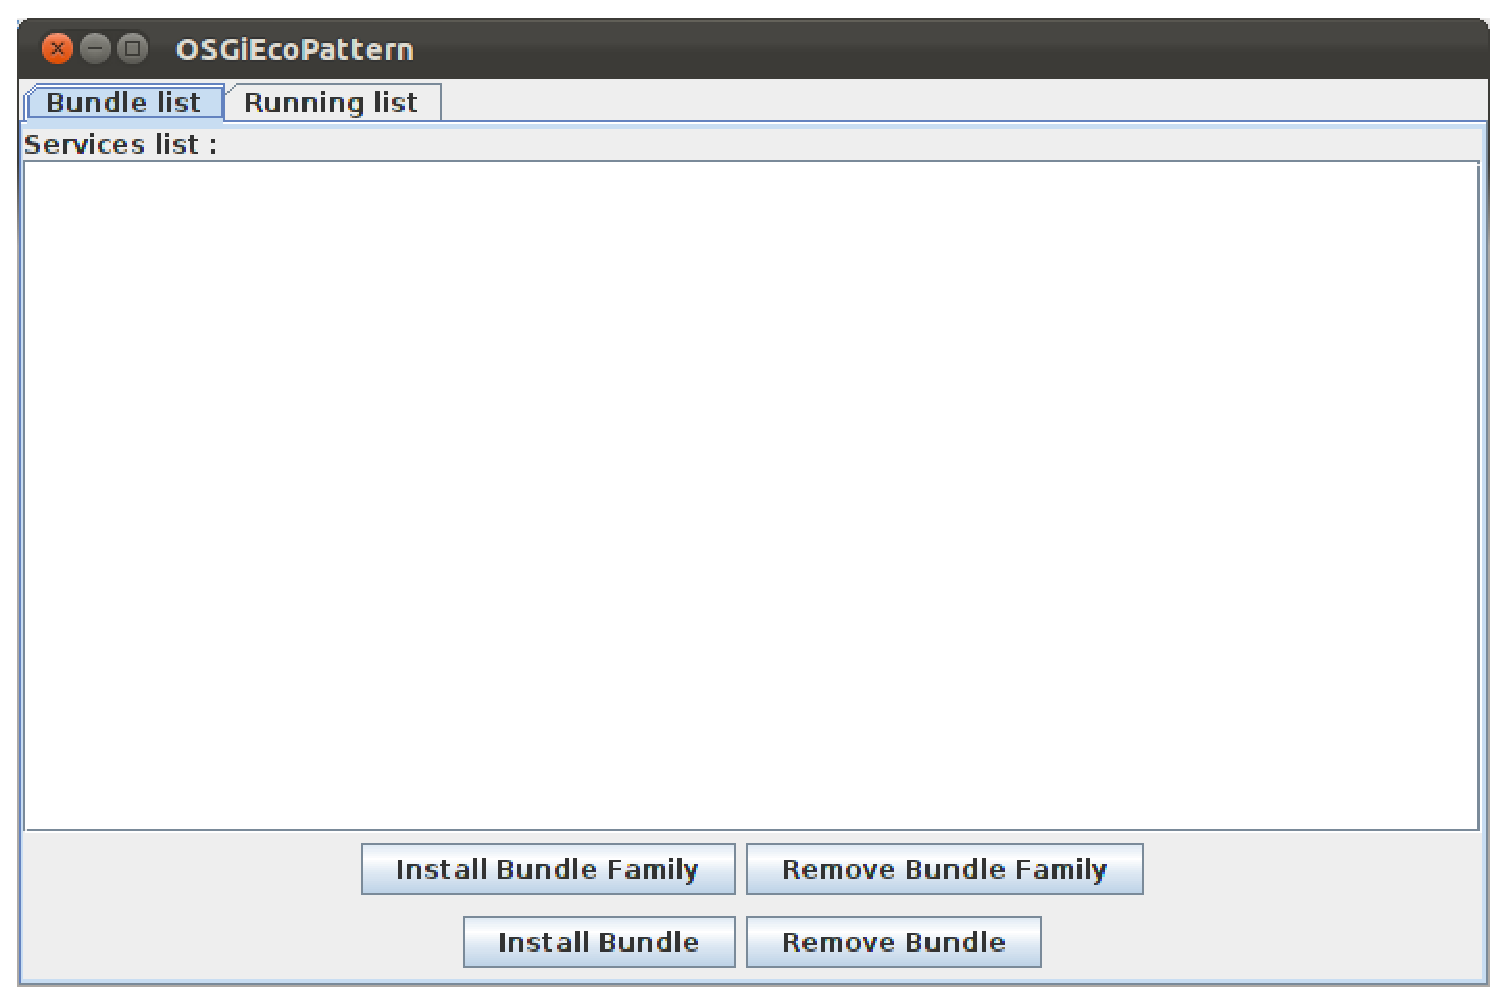
\includegraphics[width=0.95\textwidth]{figures/EcoPattern_Bundle_List_View}
	\caption{Interface d'installation des services}
	\label{BdlList}
\end{figure}
\begin{figure}
	\centering
	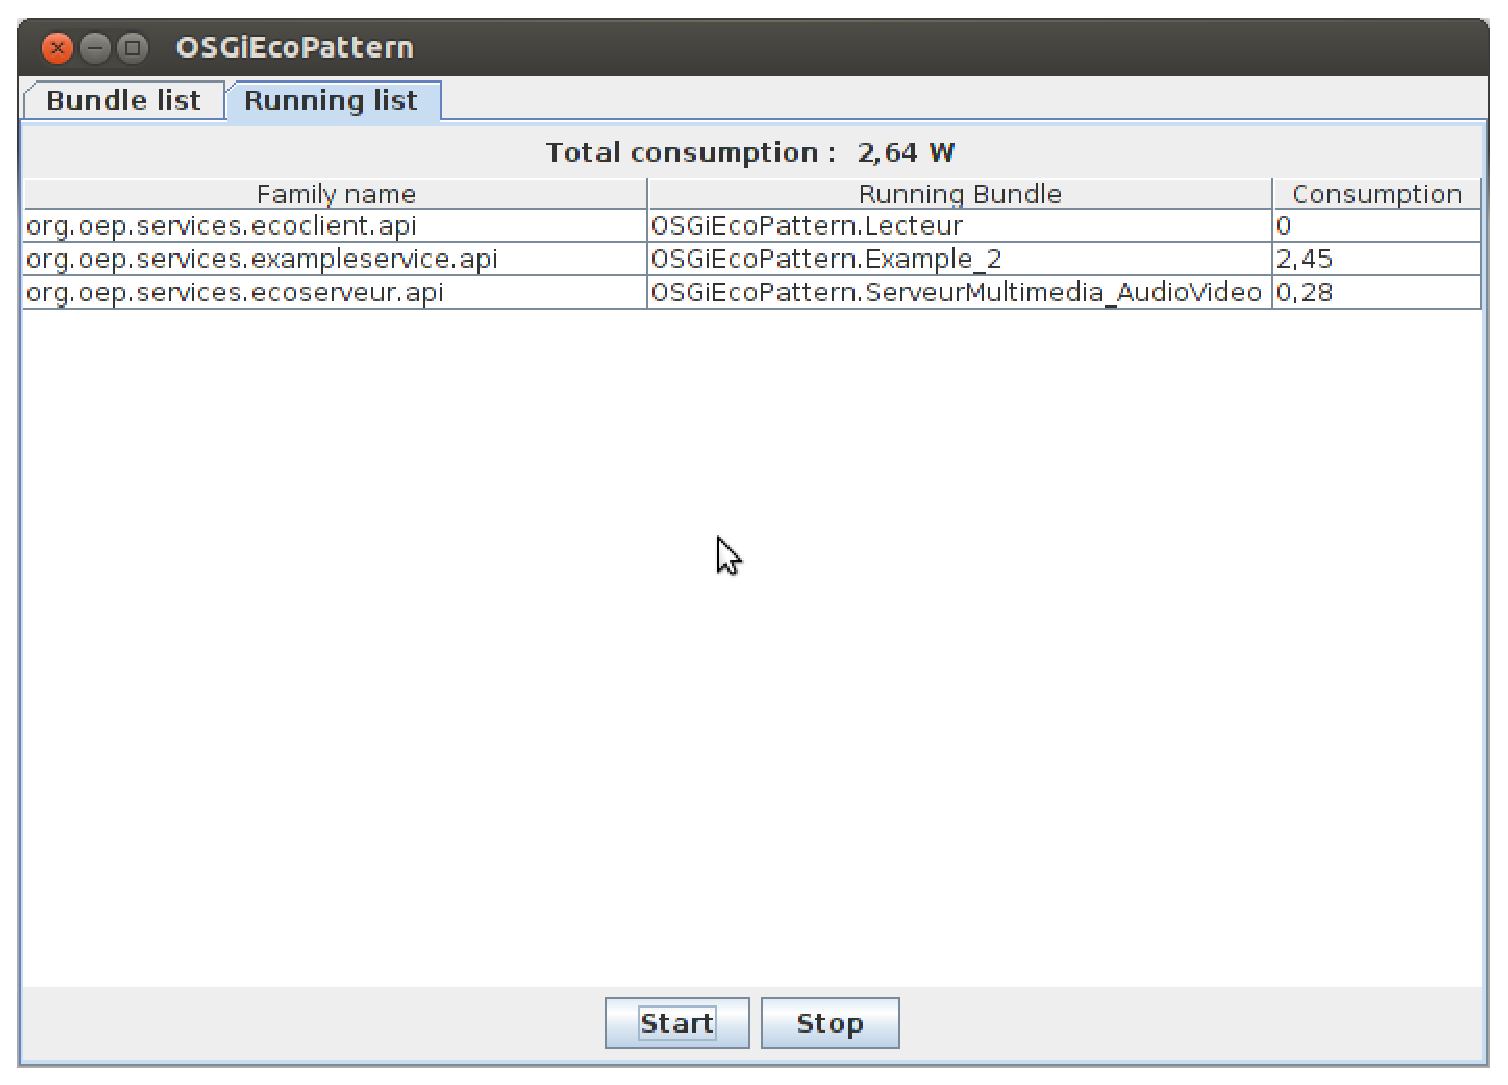
\includegraphics[width=0.95\textwidth]{figures/EcoPattern_Running_List_View}
	\caption{Interface de gestion des services démarrés}
	\label{RngList}
\end{figure}

L'interface en ligne de commande est basé sur le shell felix\footnote{http://felix.apache.org/site/apache-felix-shell.html}. J'ai défini seulement trois commandes ~:
\begin{itemize}
  \item une pour installer une famille de module
  \item une pour installer un module
  \item une pour obtenir la consommation global
\end{itemize}
Pour obtenir un shell complet, il faudrait ajouter à cela une commande pour démarrer, une commande pour arrêter et une commande pour obtenir la consommation d'un module. Je n'ai pas écrit ces commandes car j'ai choisi de privilégier l'interface graphique qui me paraissait plus pertinente pour faire des démonstrations.

En plus des interfaces utilisatrices, j'ai conçu un module qui s'occupe d'exporter les données de consommation vers un fichier \textit{CSV}. Cela permet de faire facilement des sauvegardes d'historique de consommation ou bien d'afficher en temps réél une courbe au moyen du logiciel KST.
 
		\subsection{Le controleur}
Le controleur est la partie sur laquelle j'ai pu le moins travailler. Il est charger de détecter des changements dans la consommation des modules et de déclencher une action de reconfiguration si besoin. Je souhaitais utiliser pour cela l'API \textit{Wildcat}\footnote{http://wildcat.ow2.org/}. C'est un projet de l'OW2 consortium qui a pour but de fournir un cadriciel permettant la mise en place de sondes et de déclencher des évènements au moyen de requêtes écrites dans un langage proche du SQL.

J'ai abandonné cette solution après avoir passé plusieurs jours à tenter d'intégrer Wildcat dans un module OSGi sans y arriver (ceci  à cause de problème de dépendance à d'autres bibliothèques). J'ai donc finalement opté (un peu dans l'urgence) pour une solution plus basique qui vient tester tour à tour chaque module pour vérifier qu'il ne dépasse pas une limite de consommation. Cette version du controleur ne permet pas de mettre en place une politique de consommation élaborée, mais cela m'a permis de faire fonctionner le cadriciel dans le temps imparti pour mon stage. Étant donné qu'il est totalement indépendant du reste du cadriciel, on peut facilement le remplacer par un autre plus complexe.
   
		\subsection{L'application}
L'application que l'on souhaite faire fonctionner au sein de ce cadriciel doit être basé sur la notion services. Afin d'être pris en compte, les modules de cette application doivent implémenter l'interface \textit{EcoService} présent dans le module \textit{org.oep.services.api}. Cette interface ne définit qu'une seule méthode ~:
\begin{verbatim}
        public double getConsumption();
\end{verbatim}
 qui sert à récupérer la consommation d'un module. L'interface sert aussi à catégoriser les modules comme étant intégré au cadritiel.
 
	\section{Résultats obtenus}
Afin d'illustrer les résultats obtenu par ce framework, j'ai développé une application exemple. Elle est composée de deux modules qui sont interchangeable. Ces modules ne font rien à part augmenter de façon artificielle leurs consommations en partant de 2 watts. Durant l'expérience, le controleur est programmé pour remplacer un module dès que celui ci dépasse une consommation de 3 watts. 

\begin{figure}
	\centering
	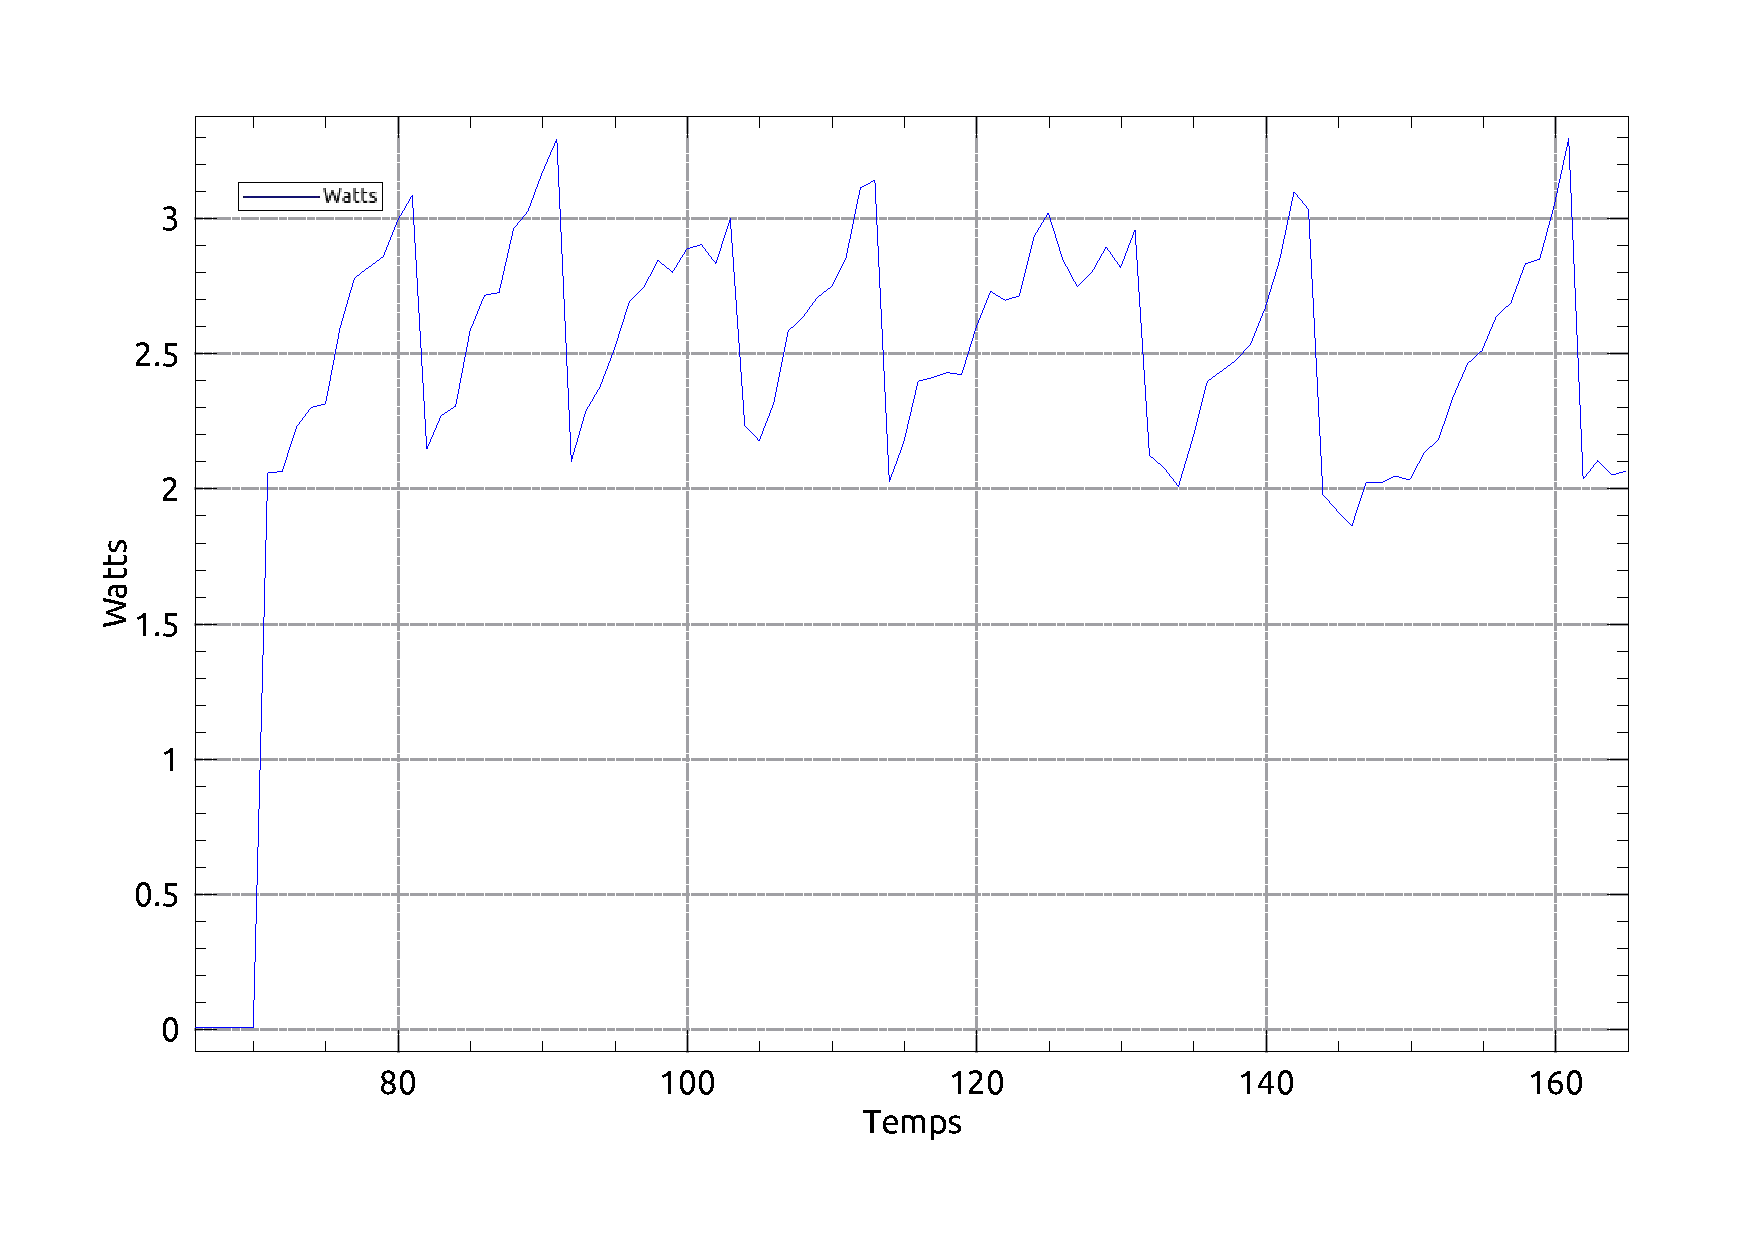
\includegraphics[width=0.95\textwidth]{figures/EcoPattern_Courbe_Exemple.pdf}
	\caption{Courbe de la consommation du programme Exemple}
	\label{CourbeExp}
\end{figure}

Ce prototype d'application provoque donc l'échange régulier des deux modules entrainant par la même une baisse de la consommation. On peut voir le résultat sur cette courbe de consommation (figure~\ref{CourbeExp}) ou l'on constate bien que régulièrement la courbe chute brutalement. Ces chutes correspondent à l'échange de module.

	\section{Développer une application pour ce framework}
Développer une application pour ce cadridiel est avant tout développer une application sous OSGi. Je ne détaille pas ici les principes de cette technologie (je l'ai déjà abordé dans mon état de l'art). On doit donc développer des modules ou \textit{bundle}. Deux types de modules doivent être fait pour que le cadriciel fonctionne ~:
\begin{itemize}
  \item ceux définissant une famille de modules
  \item ceux appartenant à une famille de modules
\end{itemize}

L'application Exemple développé dans la section précédente permet d'illustrer simplement l'utilité de ces deux type de modules. On peut voir sur la figure~\ref{BdlExp} les modules qui composent cette application. Comme son nom l'indique, le module \textit{Famille\_Exemple} défininit la famille de modules auquelle appartiennent les deux autres modules.

\begin{figure}
	\centering
	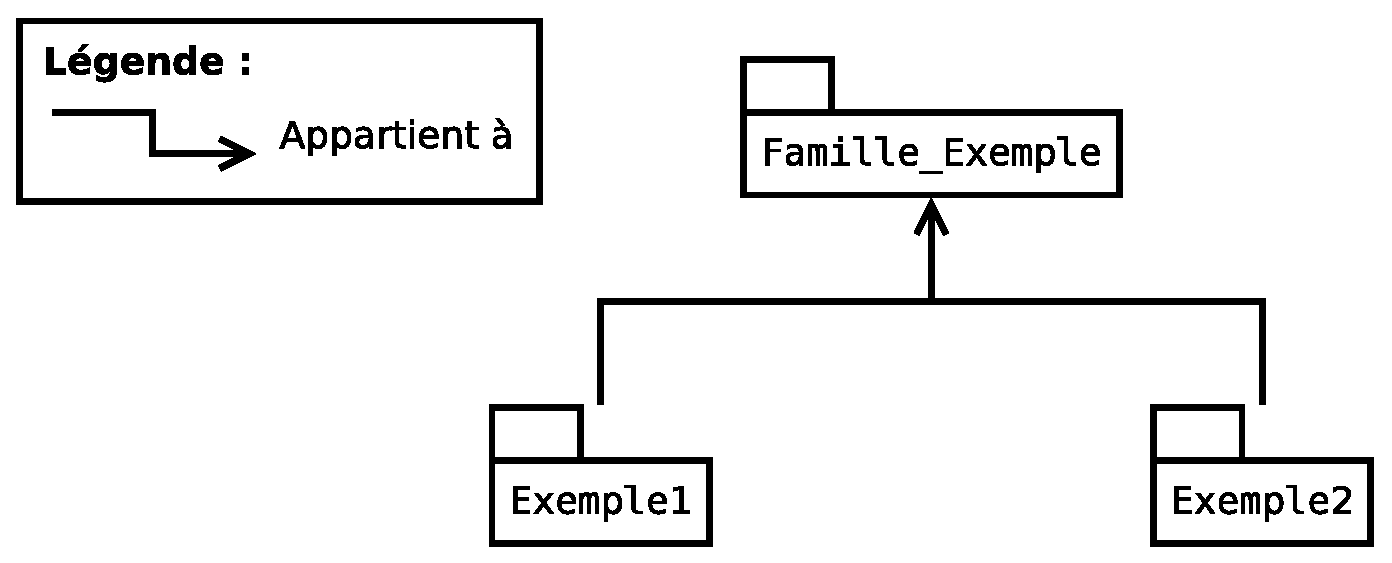
\includegraphics[width=0.55\textwidth]{figures/EcoPattern_Exemple}
	\caption{Diagramme des modules de l'application Exemple}
	\label{BdlExp}
\end{figure}

Pour voir plus en détail comment faire, le module \textit{Famille\_Exemple} contient une interface héritant de \textit{EcoService}. Les deux autres modules contiennent sensiblement la même chose, à savoir une classe implémentant l'interface définit dans le module \textit{Famille\_Exemple}.

	\section{Un exemple d'application ~: lecteur audio}
Afin d'illustrer les possibilités de ce framework, j'ai développé un exemple concret d'application. Cette application est un simple lecteur multimedia. Sa particularité est que quand on a besoin d'économiser l'énergie il n'affiche plus l'image et ne diffuse que le son du fichier numérique que l'on souhaite lire. Ce lecteur est basé sur la bibliothèque Java Xuggle\footnote{\href{http://www.xuggle.com/}{www.xuggle.com}}.

L'architecture de cette application (figure~\ref{lecMult}) est divisé en deux familles de modules. La première, définit par le module \textit{Famille\_Lecteur}, fournit l'interface graphique du lecteur multimedia. Pour cet exemple, je n'ai développé qu'une version contenu dans le module \textit{Lecteur}. La deuxième famille est celle définit dans le module \textit{Famille\_ServeurMultimedia}. Elle sert à charger, décoder et lire le fichier multimédia. Pour cette famille j'ai développé deux modules. Le module \textit{LecteurMultimedia\_AudioVideo} qui décode et affiche les flux audio et vidéo du fichier. L'autre, le module \textit{LecteurMultimedia\_Audio}, ne s'occupe que de la partie Audio du fichier.

\begin{figure}
	\centering
	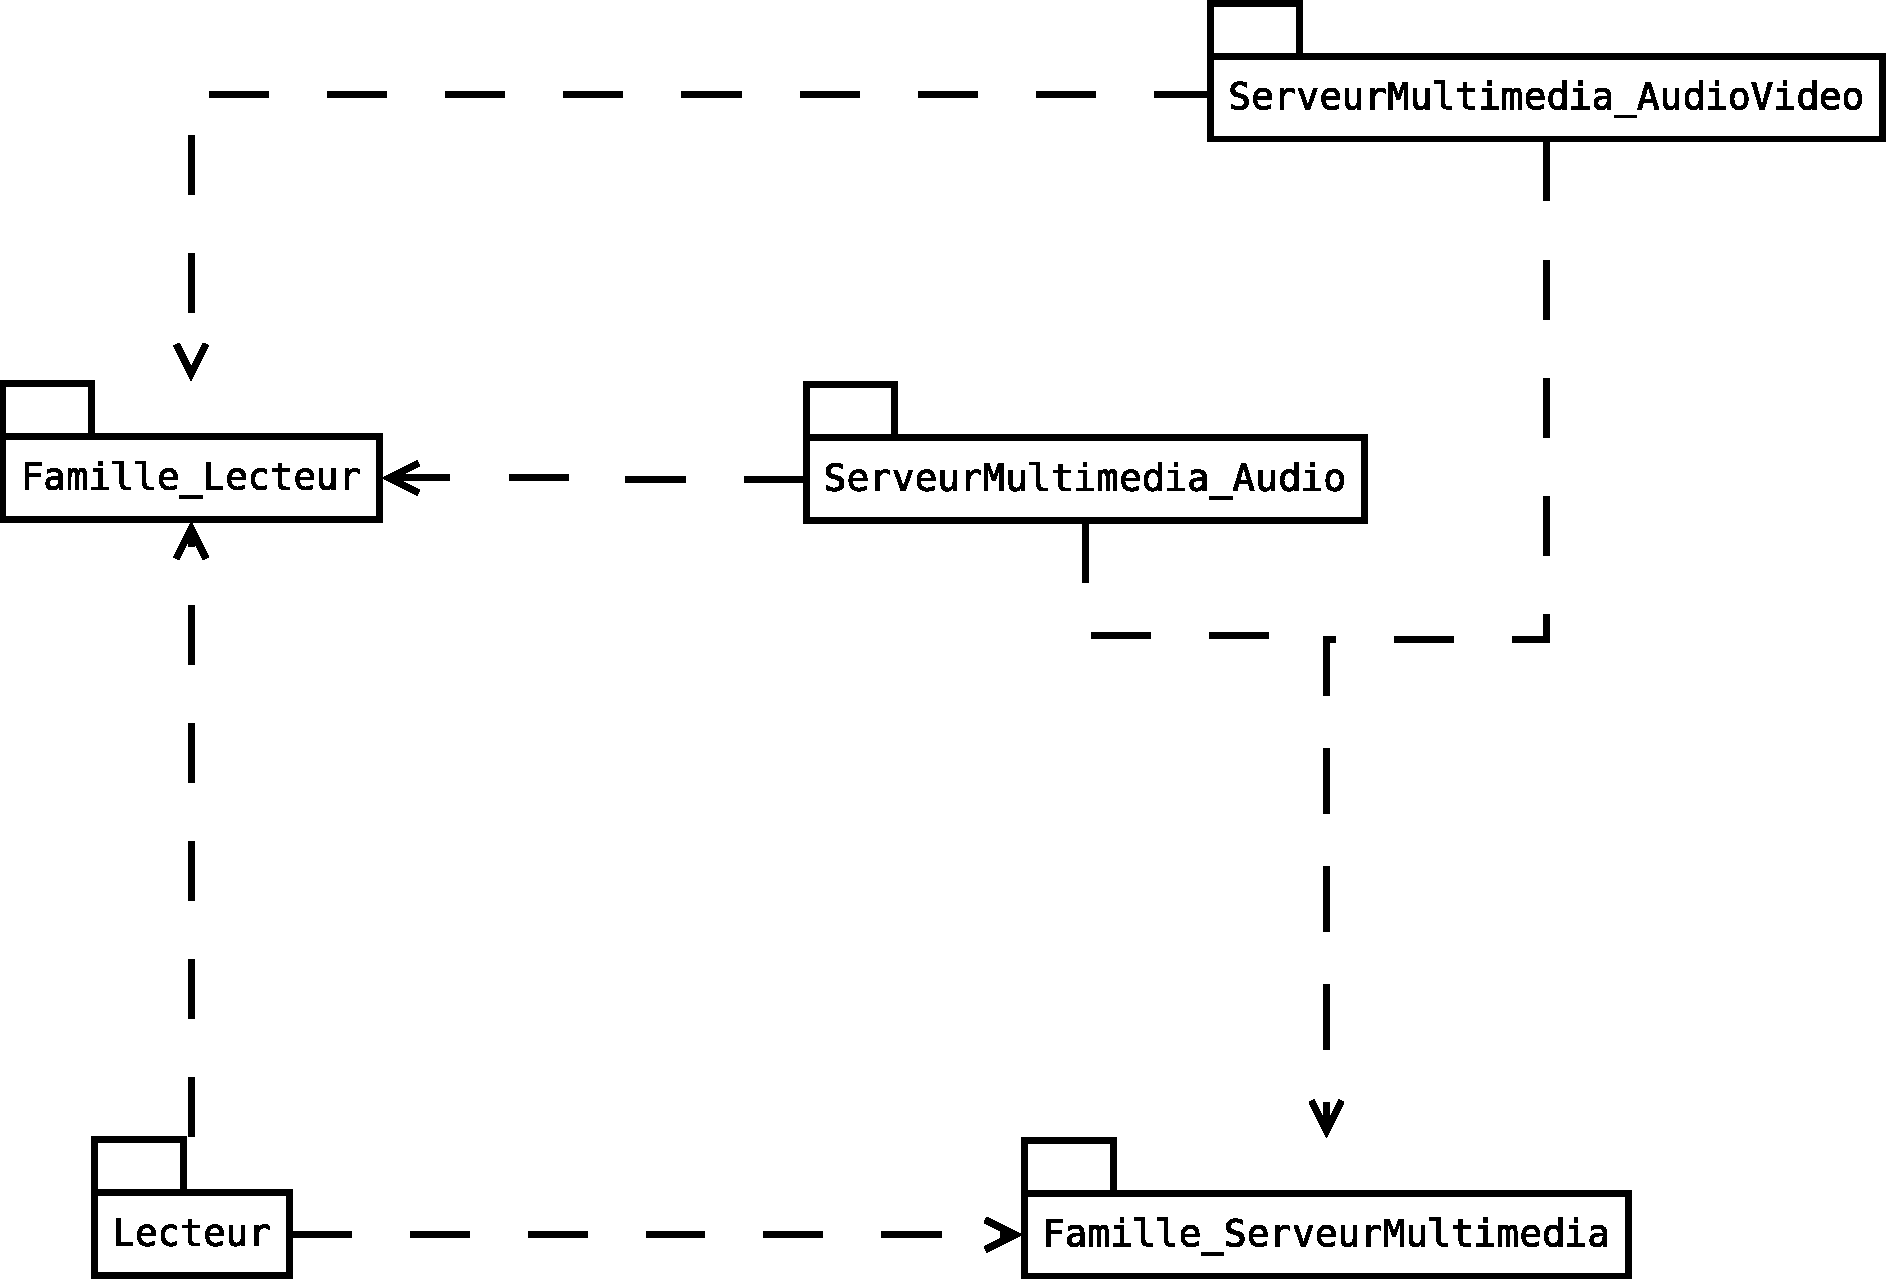
\includegraphics[width=0.95\textwidth]{figures/EcoPattern_LecteurMultimedia}
	\caption{Lecteur multimedia ~: Diagrammame de liaison des modules}
	\label{lecMult}
\end{figure}

Au final, nous avons donc un module qui rend une qualité de service supérieur mais qui consomme plus (11,5 watts mesuré avec un wattmètre) et l'autre qui dégrade la qualité de service, en supprimant le traitement de la vidéo, pour consommer moins (4,2 watts mesuré avec un wattmètre).

\chapter{Conclusion}
Voici donc l'ensemble du travail que j'ai pu effectuer durant mon stage de fin d'étude. Il reste encore beaucoup de travail pour pouvoir obtenir des résultats concrets et enfin pouvoir dire que l'on sait éco-concevoir un logiciel. Cinq mois furent trop courts pour pouvoir développer l'ensemble des idées que je souhaitais aborder. J'ai du faire des choix et cibler mon étude.

Pour moi, ce fut un travail passionnant. Je suis heureux d'avoir eu l'opportunité de travailler dans de telle condition. J'ai pu apprendre beaucoup de nouvelles technologies à commencer par OSGi ou Wildcat. J'ai aussi beaucoup appris sur des mécanismes de systèmes et sur le fonctionnement de certains langages. J'ai débuté mon stage en étant convaincu de l'utilité de ce type de démarche, j'en ressors en pensant que c'est une nécéssité.

\bibliographystyle{plain}
\bibliography{biblio}
\listoffigures{}
\listoftables{}
\appendix

\chapter{Sujet de stage}
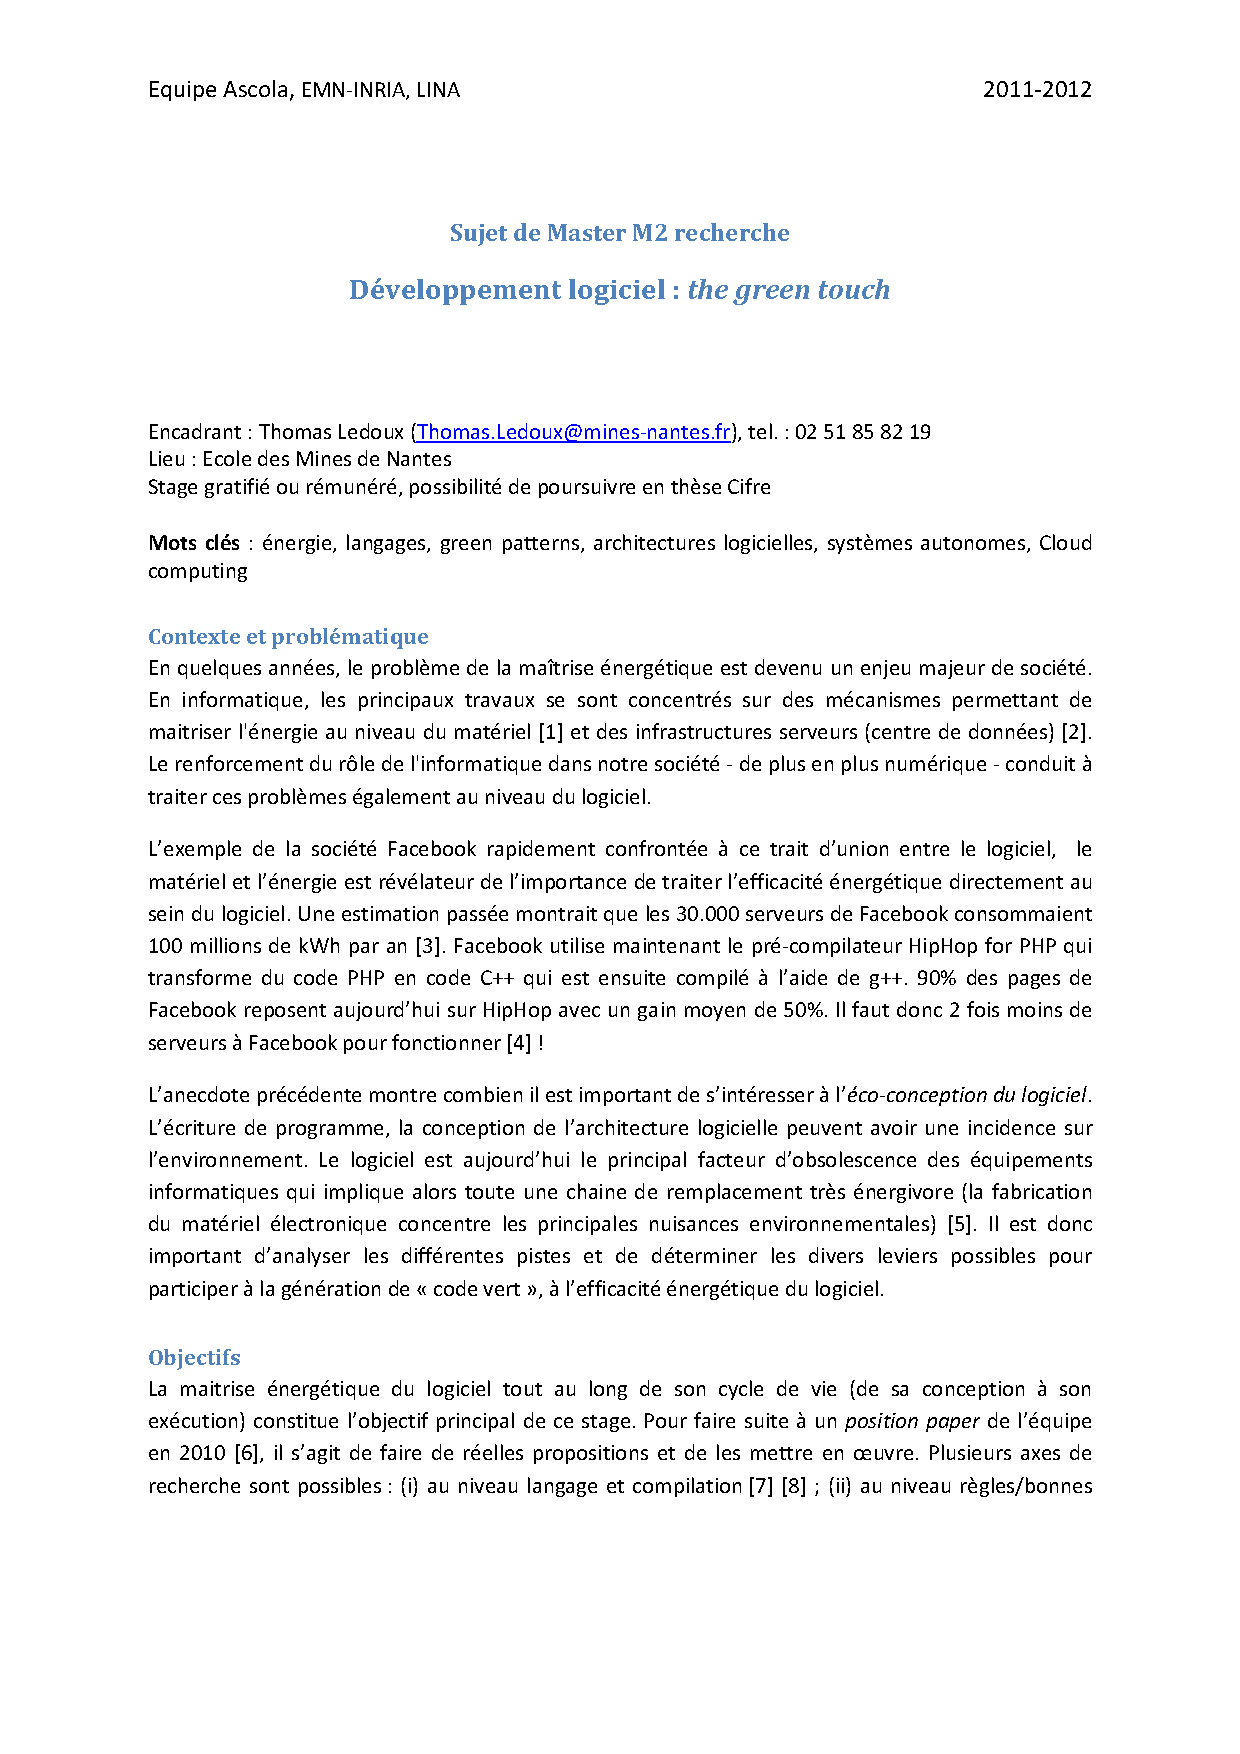
\includepdf[lastpage=3,pages=1]{imports/Sujet_Master_EcoConceptionGL.pdf}
\includepdf[lastpage=3,pages=2]{imports/Sujet_Master_EcoConceptionGL.pdf}
\includepdf[lastpage=3,pages=3]{imports/Sujet_Master_EcoConceptionGL.pdf}

\chapter{Plannification}
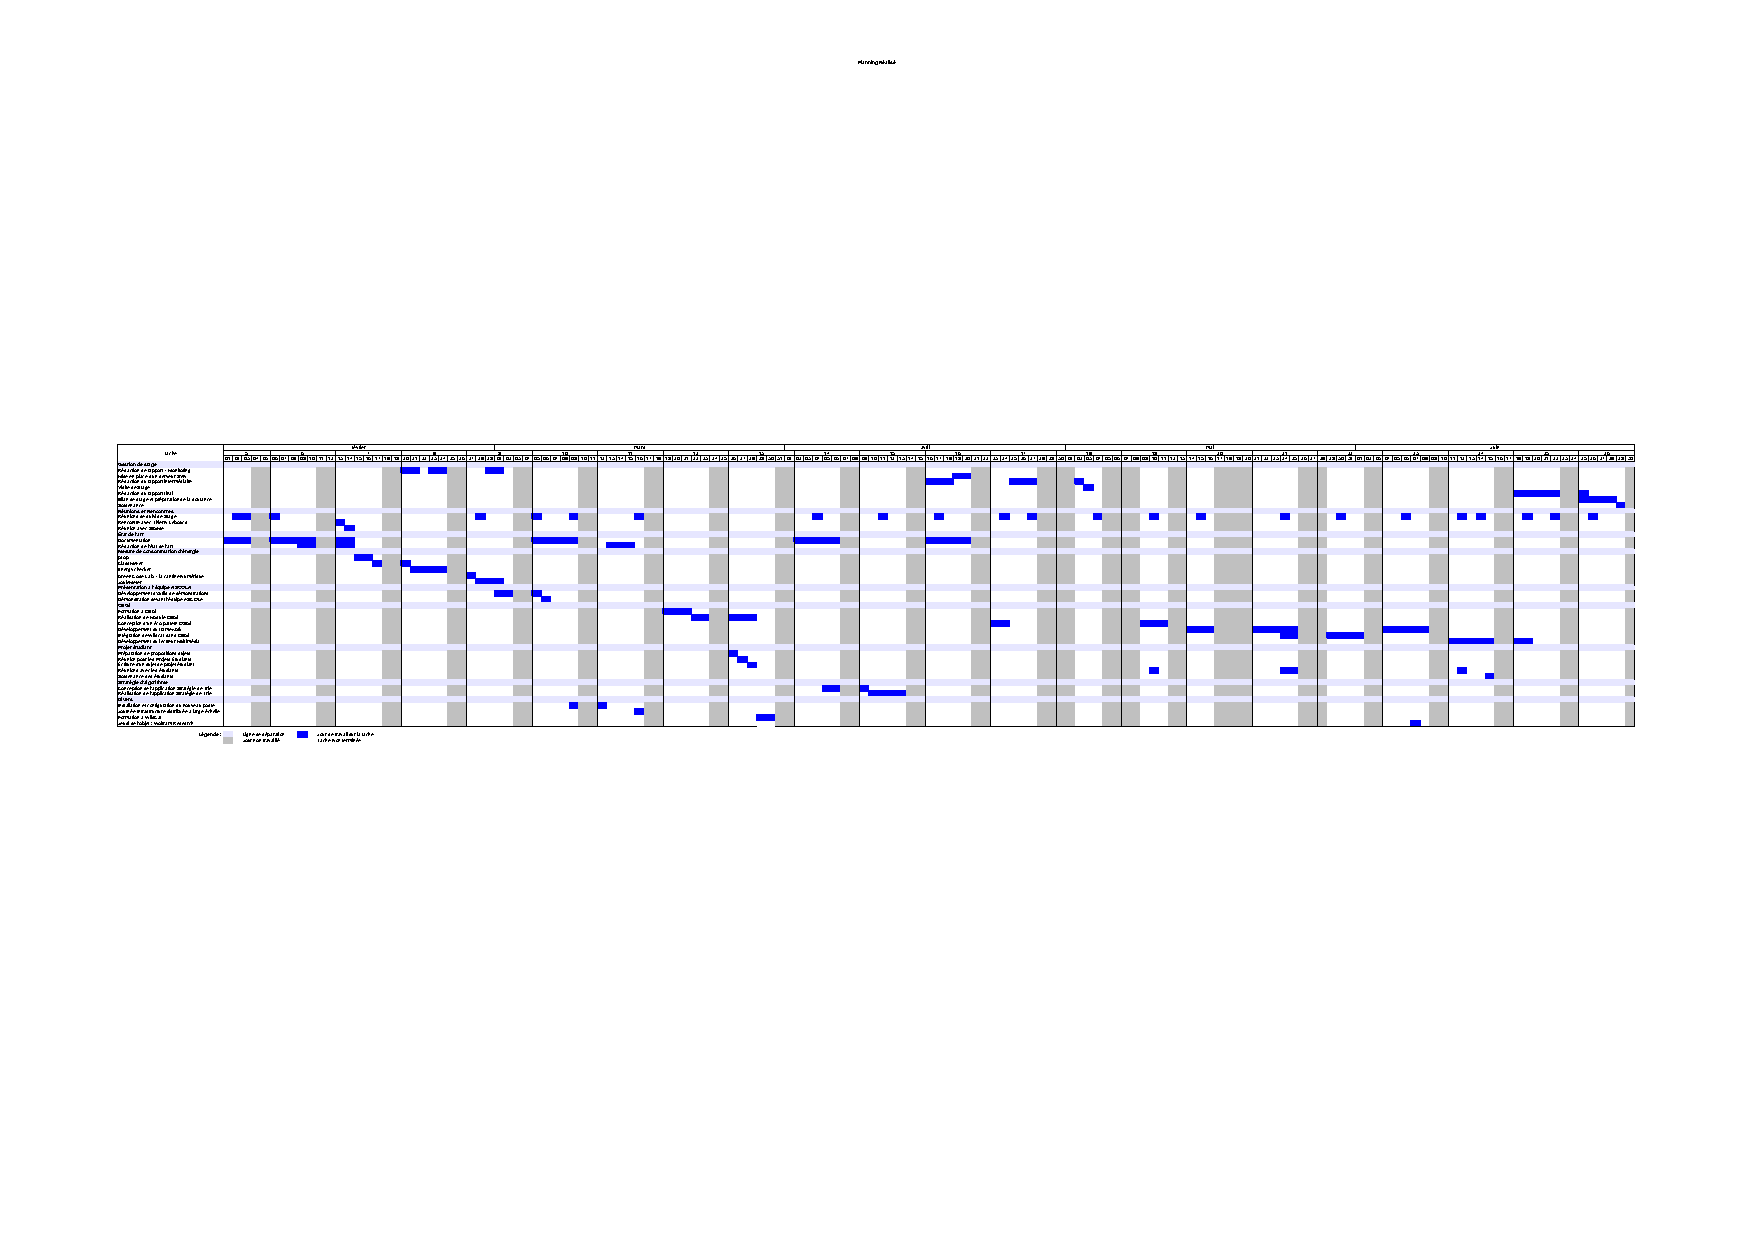
\includepdf[lastpage=2,pages=1,angle=90]{imports/Planning_realise_finale.pdf}

\chapter{Diagrammes de Classes d'EcoFramework}
\section{Package org.oep.core}
	\begin{centering}
		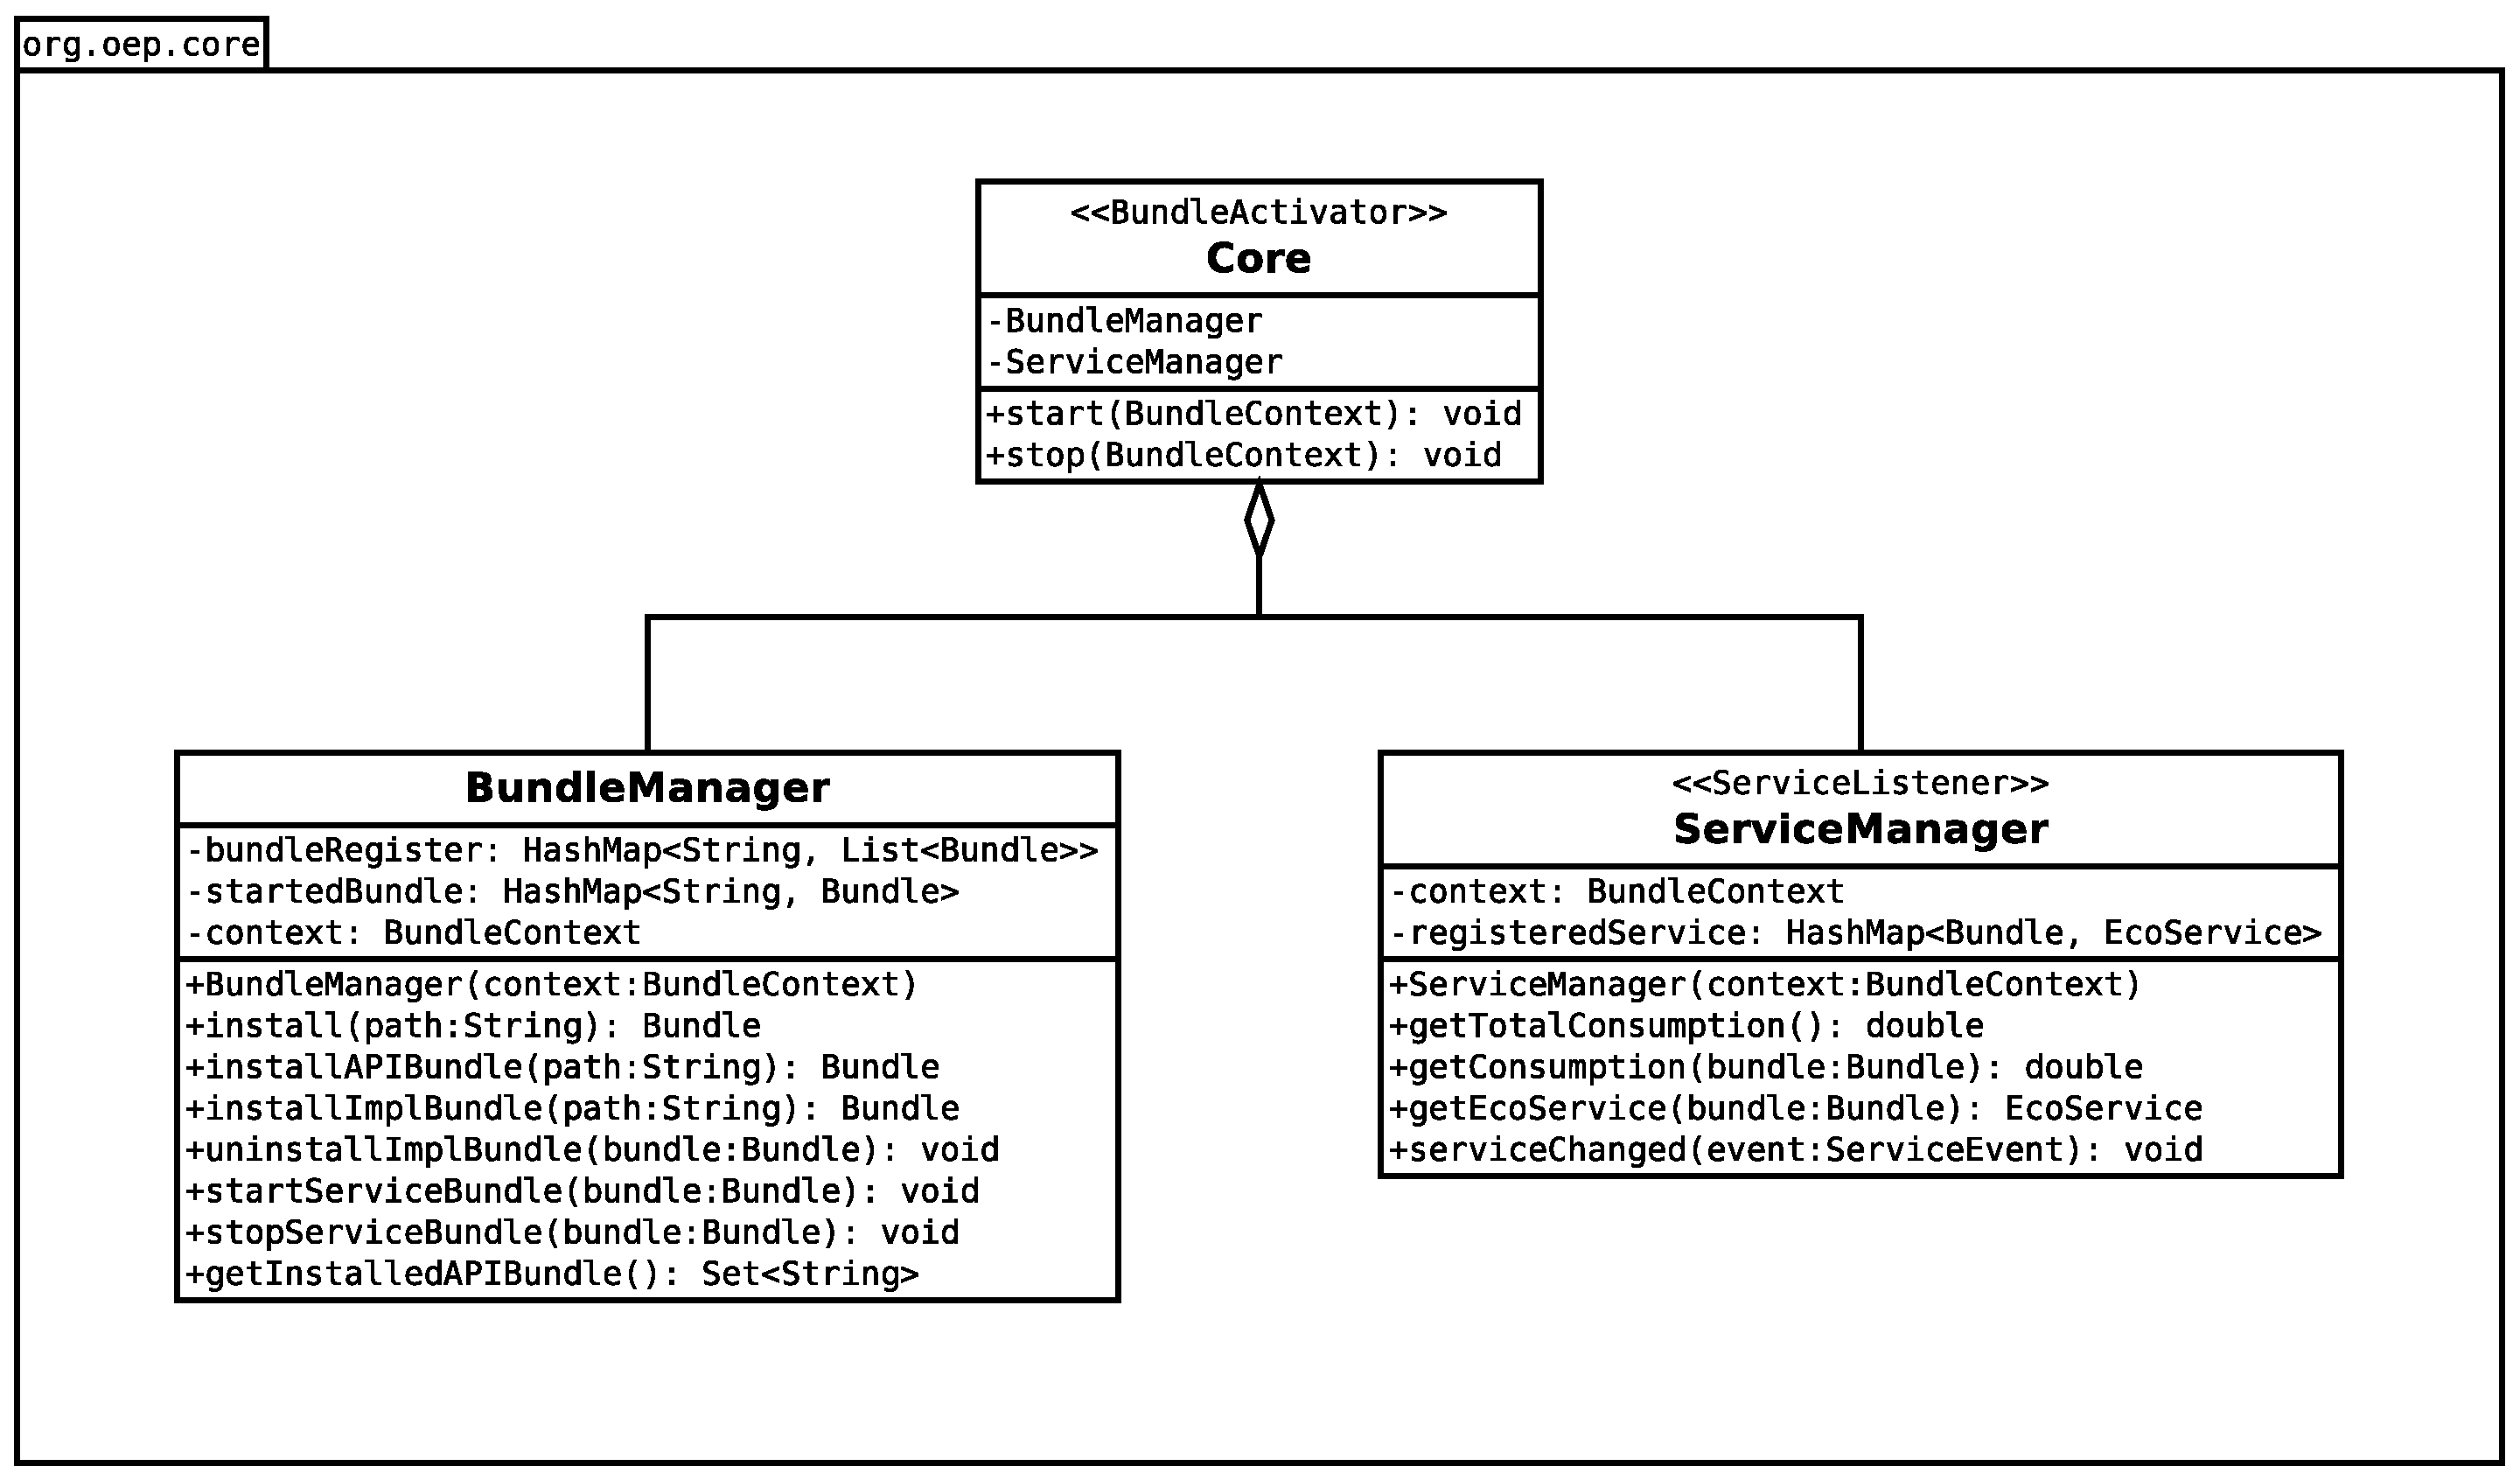
\includegraphics[width=0.99\textwidth]{figures/EcoPattern_Core_Classes}
	\end{centering}
\section{Package org.oep.shell}
	\begin{centering}
		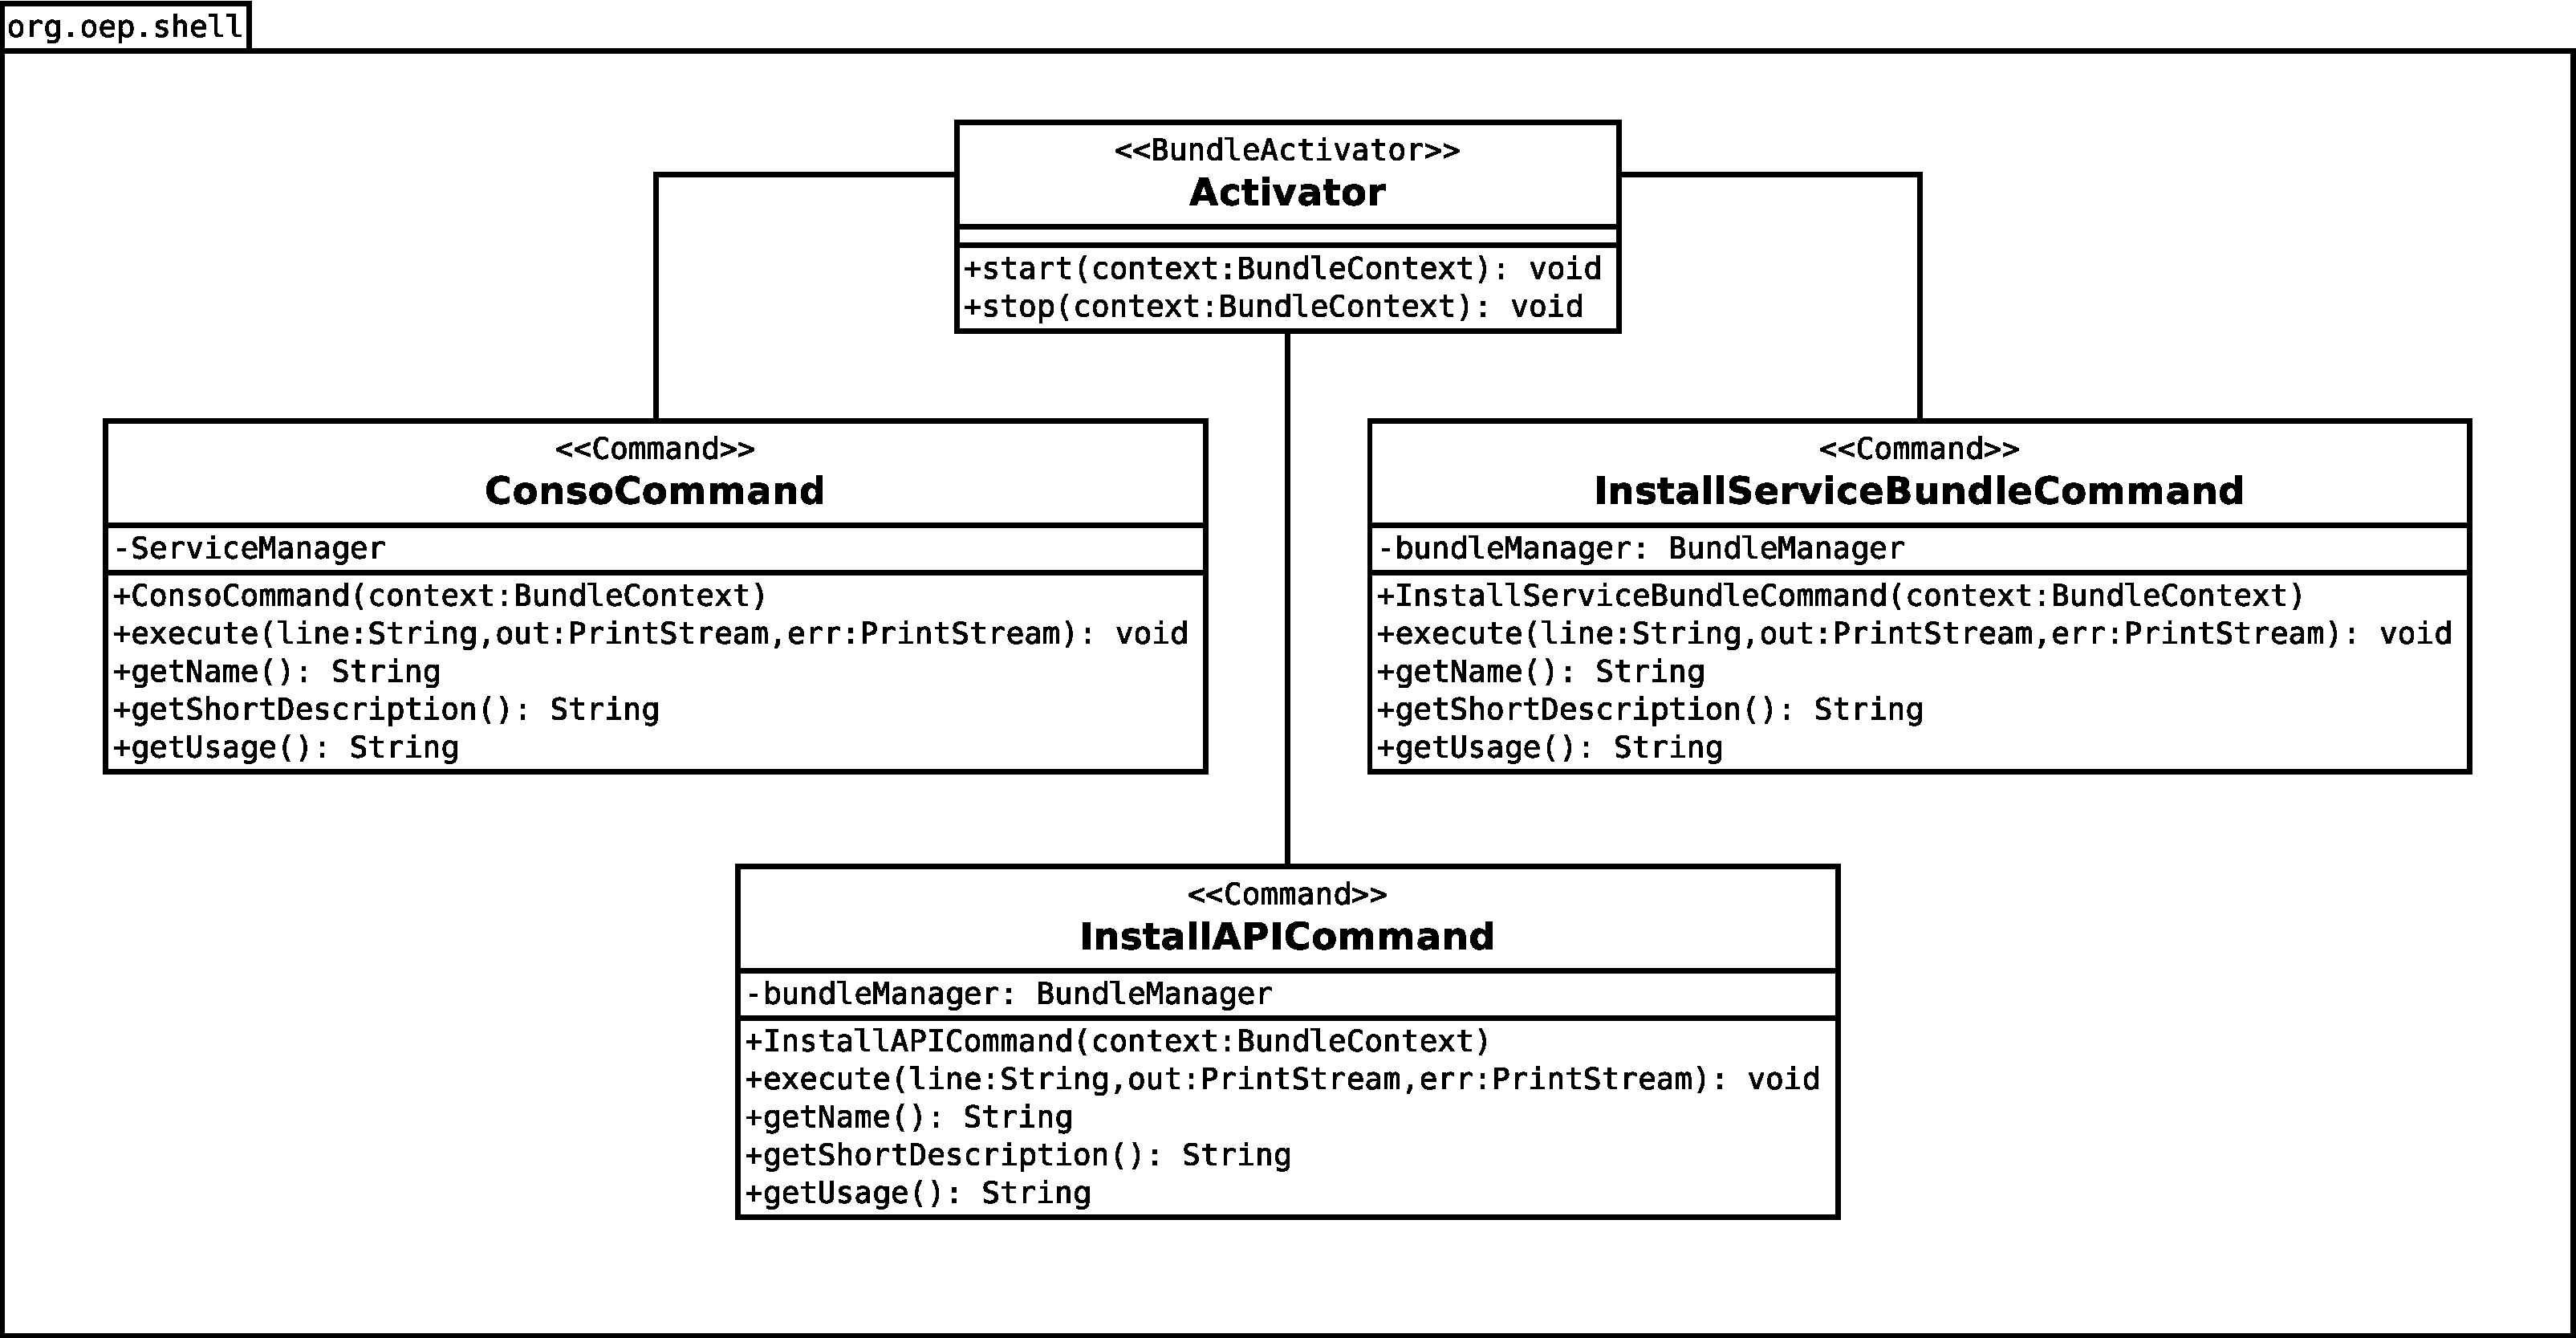
\includegraphics[width=0.99\textwidth]{figures/EcoPattern_Shell_Classes}
	\end{centering}
\section{Package org.oep.gui}
	\begin{centering}
		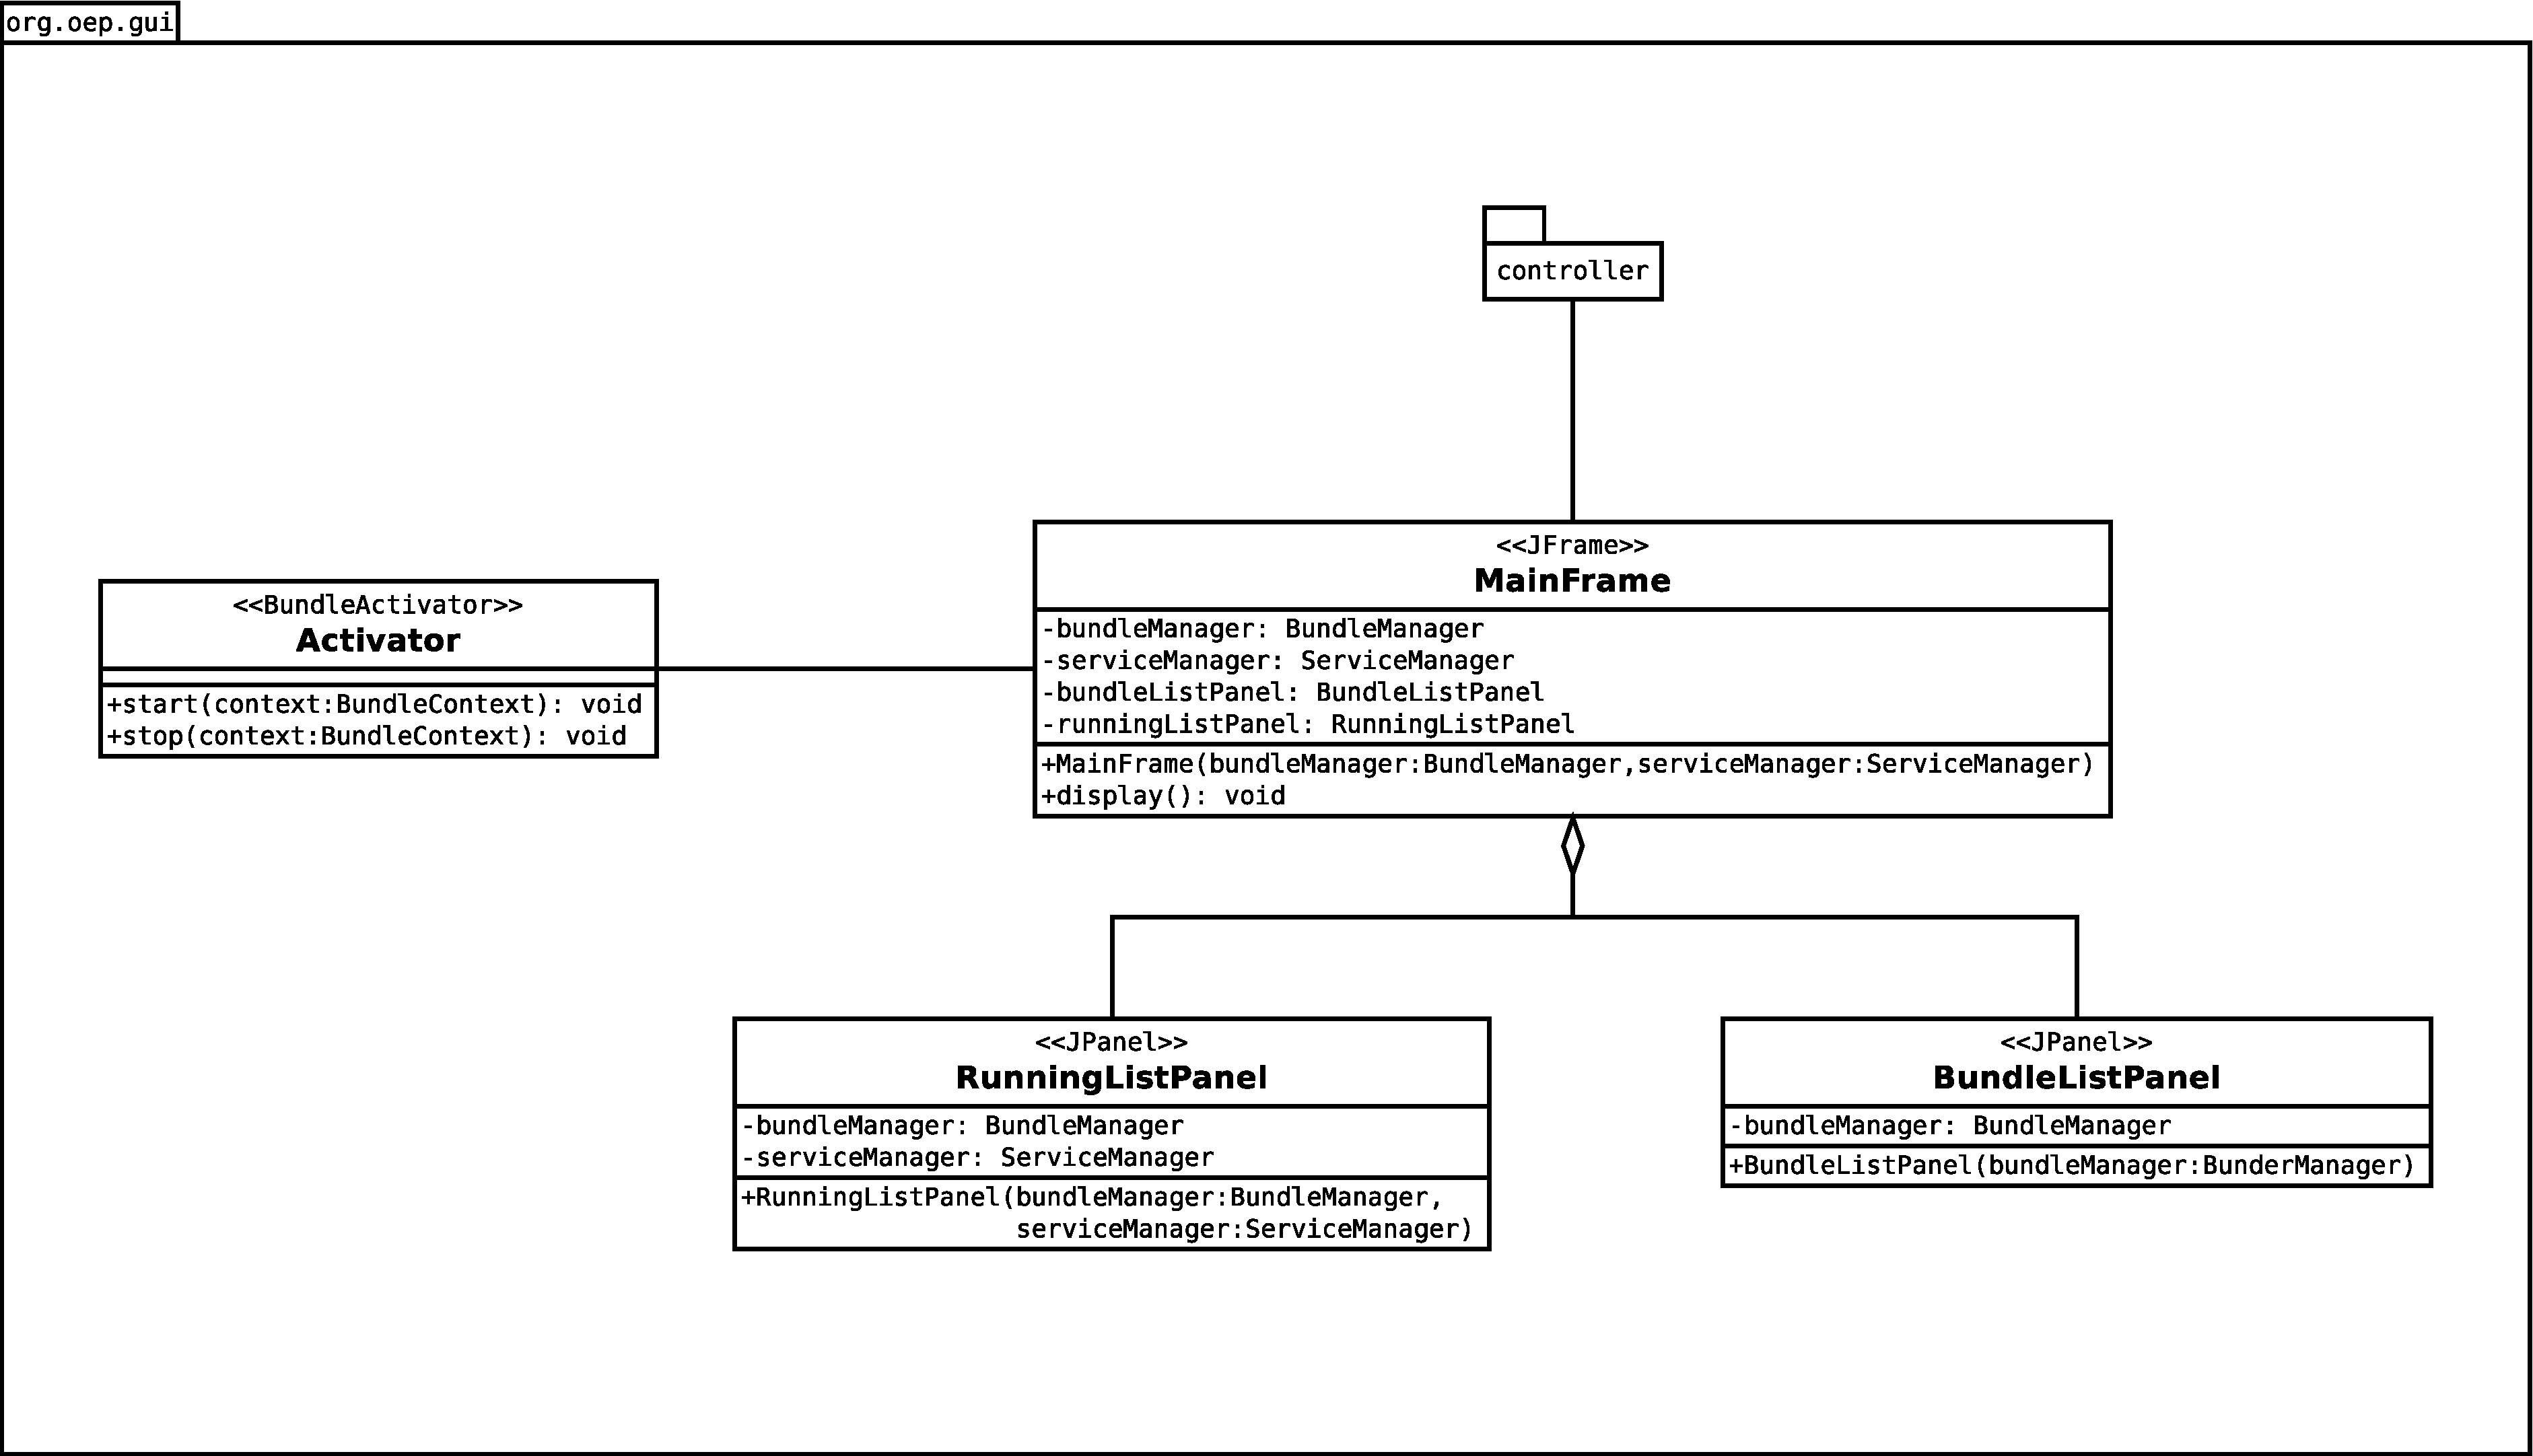
\includegraphics[width=0.99\textwidth]{figures/EcoPattern_Gui_Classes}
	\end{centering}
\section{Package org.oep.core.controller.basic}
	\begin{centering}
		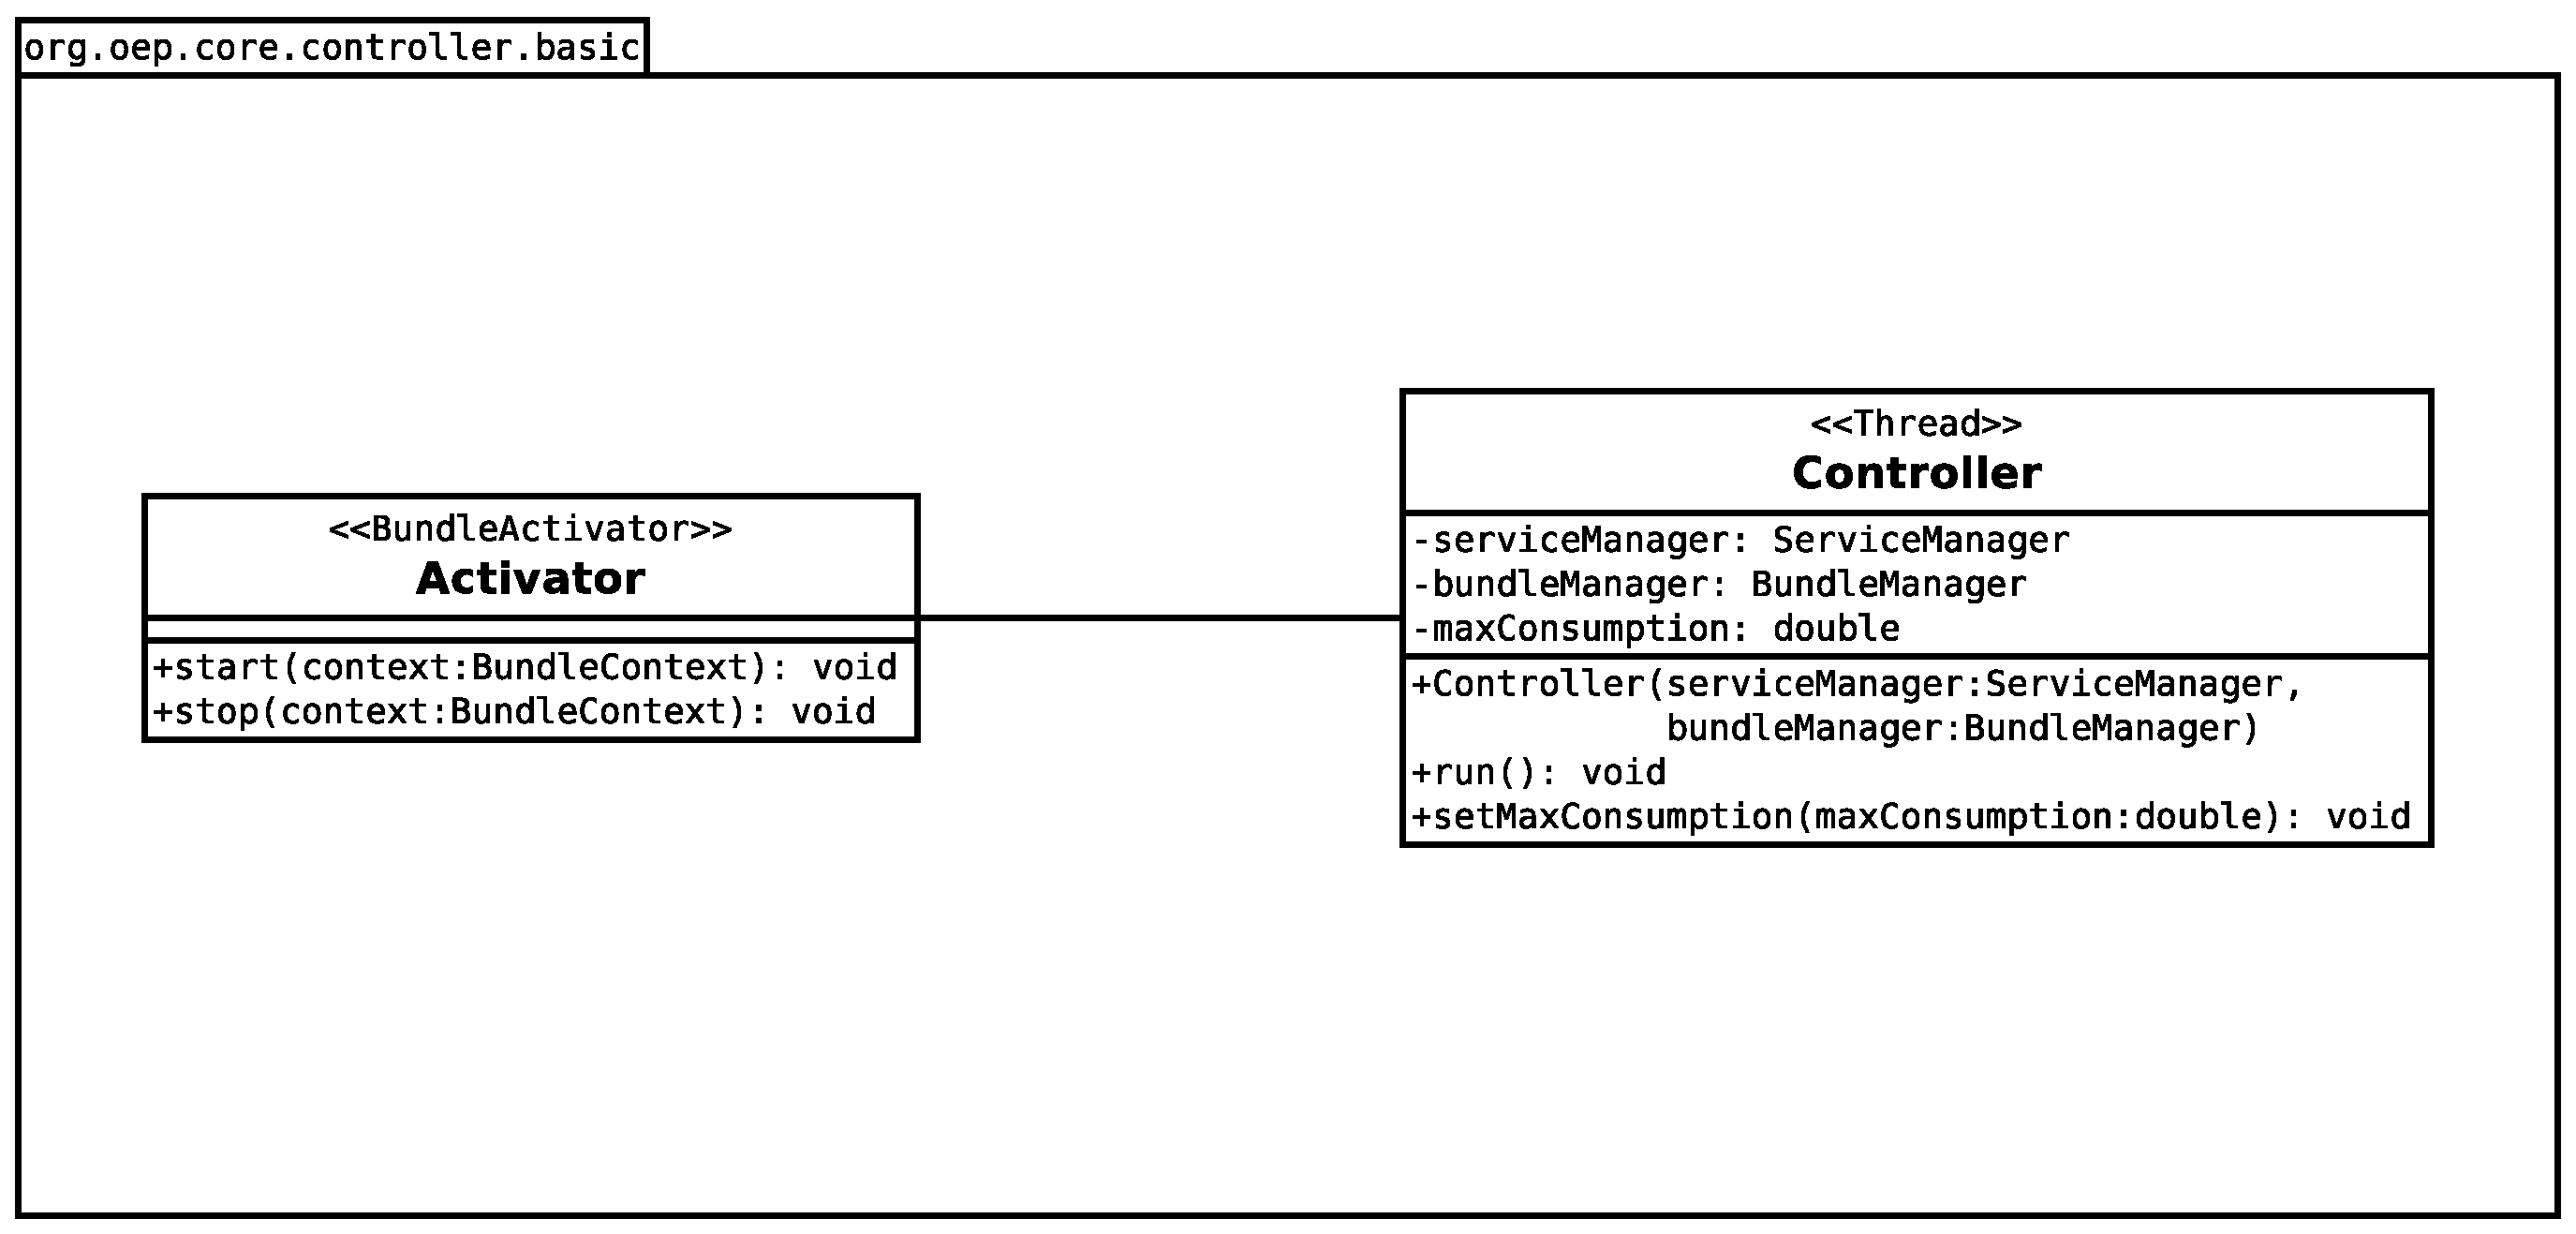
\includegraphics[width=0.99\textwidth]{figures/EcoPattern_Controller_Basic_Classes}
	\end{centering}
\section{Package org.oep.service.api}
	\begin{centering}
		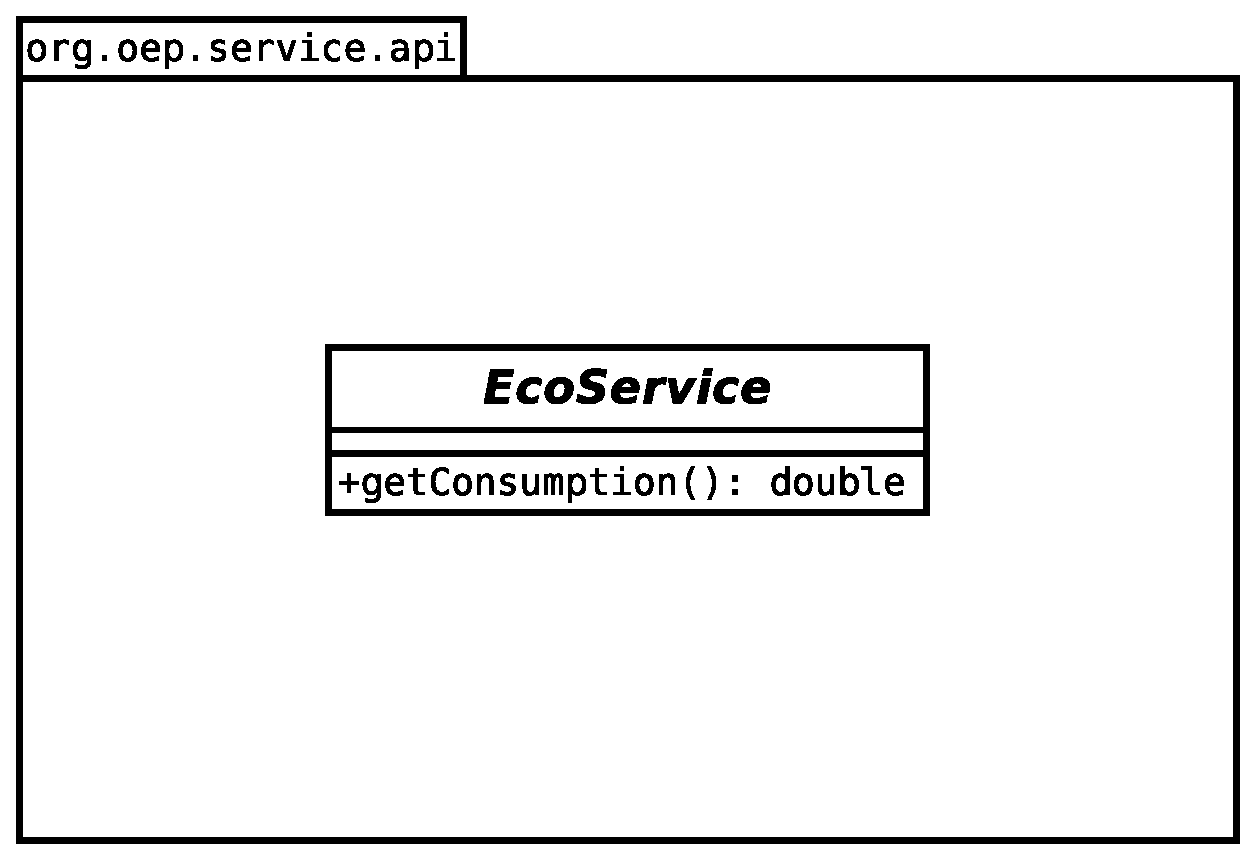
\includegraphics[width=0.45\textwidth]{figures/EcoPattern_Service_Api_Classes}
	\end{centering}
\end{document}